\documentclass[oneside]{fduthesis}%打印用twoside,电子版用oneside
\usepackage{mymacro}
\graphicspath{{figures/}}
\begin{document}
%%%%%%%%%%%%%%%%%%%%%%%%%%%%%%
%% 封面部分
%%%%%%%%%%%%%%%%%%%%%%%%%%%%%%
\makefrontcover{13110180026}%学号
{基于多任务和组稀疏的子空间聚类方法}% 中文标题
{Subspace Clustering via Multitasking and Group Sparsity}%
{数学科学学院}%
{计算数学}%
{张\hspace{1em}航}%
{张淑芹\hspace{1.5em}副教授}%
{2016年4月1日}
%扉页
\makeheadpage{张淑芹\hspace{1.5em}副教授}%
{高卫国\hspace{1.5em}教\hspace{1em}授}
{张淑芹\hspace{1.5em}副教授}
%特别注意,以下述顺序为准,在对应部分添加文档部件,切勿颠倒顺序:
%论文的文档部件顺序是:
%    frontmatter:目录、中文摘要、英文摘要、符号说明
%    mainmatter: 正文章节
%    backmatter: 参考文献、附录、致谢、声明
%%%%%%%%%%%%%%%%%%%%%%%%%%%%%%
%% 前言部分
%%%%%%%%%%%%%%%%%%%%%%%%%%%%%%
\frontmatter
% 目录
\tableofcontents
%\listoffigures
%\listoftables
% 摘要
\begin{cnabstract}
  在大数据时代, 我们面对海量高维数据, 它们来自图片、视频、文字、网页等等.
  这些高维数据常常分布在多个混合的低维子空间中,
  子空间聚类就是要将一群来自不同低维子空间的数据点按照它们
  所属的空间分开, 将同一子空间的点聚成一类.
  人们提出了很多子空间聚类方法, 目前公认表现最好的是稀疏子空间聚类
  (Sparse subspace clustering, SSC). 本文在SSC的基础上,
  拓展出了基于多任务和组稀疏的新方法.
  SSC将每个数据点用其它点表示, 用表示系数构造邻接矩阵,
  进而用谱聚类分割邻接图.
  不同于SSC, 我们先利用点的局部信息, 将其分成一个个小组,
  每个小组作为一个整体, 使它们被同时表示, 或同时用来表示其它点.
  这样既可以减少只使用一个点带来的不稳定, 又能使随后生成的
  邻接图相对稠密, 正确连接较多, 从而提升聚类准确度.
  我们通过理论分析,得出新方法在一定条件下能够保证生成的邻接图
  没有错误连接, 并在Hopkins 155和NUS-WIDE数据集上与经典子空间聚类方法比较,
  验证其有效性.
  
  \keywords{高维数据\enskip 子空间聚类\enskip 无监督学习\enskip 凸优化 \enskip 多任务\enskip 组稀疏}{O24}
\end{cnabstract}

\begin{enabstract}
  In subspace clustering, a group of data points belonging
  to a union of subspaces are assigned membership to their
  respective subspaces. This paper presents a novel method
  that regularizes sparse subspace representation by exploiting the
  structural sharing between tasks and data points via multitasking
  and group sparsity. By doing this, our algorithms are able to be more robust
  without introducing much additional computational cost. The
  theoretical analysis in this paper shows that under certain conditions
  exact clustering performance can be guaranteed. We demonstrate
  the advantage of the framework on Hopkins 155 dataset and NUS-WIDE dataset.

  \enkeywords{High-dimensional data, subspace clustering, unsupervised learning, convex programming, multitasking, group sparsity}{O24}
\end{enabstract}
%此文件中含有中英文摘要

%符号说明
\begin{denotation}
\item[\(\cA, \cB, \ldots\)] 集合
\item[\(|\cA|\)] 集合\(\cA\)中的元素个数
\item[\(\S^{d-1}\)] \(\R^d\)中的单位球
\item[\(\cS\)] \(\R^d\)中的子空间
\item[\([k\char"005D\)] 若\(k\)是正整数,\([k]:=\left\{ 1, 2, \ldots,k \right\}\)
\item[\(\cI, \Omega\)] 指标集\(\cI\subset [n]\)和多个指标集组成的指标集族\(\Omega\)

\item[\(a, b, \ldots\)] 向量
\item[\(A, B, \ldots\)] 矩阵 
\item[\(a^T, A^T\)] \(a\)和\(A\)的转置 
\item[\(\mathbf{0}\)] 全为零的向量或矩阵 
\item[\(\diag(A)\)] 矩阵\(A\)的对角线向量
\item[\(\P_\cS\)] 子空间\(\cS\)的投影矩阵
\item [\([a\char"005D_i \)] 向量\(a\)的第\(i\)个元素
\item[\(A_i, A_{(i)}\) ] 矩阵\(A\)的第\(i\)列或第\(i\)行
\item[\(A_{i, j}\) ] 矩阵\(A\)的第\(i\)行第\(j\)行的元素
\item[\(a_{\cI}, A_{\cI}\)] 指标集\(\cI\)对应元素组成的向量, 以及\(\cI\)对应的列组成的矩阵 
\item[\(A_{(\cI)}\)] 以及\(\cI\)对应的行组成的矩阵 
\item[\(A_{\cI, \cJ}\)] 将\(A\)行按指标集\(\cI\)抽出, 列按指标集\(\cJ\)抽出组成的子矩阵. 
\item[\(A_\cI^T, A_{(\cI)}^T\)] 先取出\(\cI\)对应的子矩阵, 再转置
\item[\(A_{\cI\rightarrow 0}\)] 将矩阵\(A\)对应指标集\(\cI\)的列置为零

\item[\(\|a\|_2, \|A\|_F\)] \(a\)的\(\ell_2\)范数和\(A\)的Frobenius范数
\item[\(\|a\|_1, \|A\|_1\) ] \(a\)和\(A\)的\(\ell_1\)范数,即\(\|a\|_1:=\sum_i |[a]_i|, \|A\|_1:=\sum_i \|A_i\|_1\) 
\item[\(\|a\|_\infty, \|A\|_\infty\)] \(a\)和\(A\)的\(\ell_\infty\)范数,即\(\|a\|_\infty:=\max_i |[a]_i|, \|A\|_\infty:=\max_i \|A_i\|_\infty\) 
\item[\(\|A\|_2\)] \(A\)的诱导范数,即\(\|A\|_2:=\max_{\|v\|_2 = 1} \|Av\|_2\)
\item[\(\|A\|_{2,1}\) ] \(A\)每列的\(\ell_2\)范数求和,即\(\|A\|_{2,1}:=\sum_{i} \|A_i\|_2\) 
\item[\(\|A\|_{2,\infty}\) ] \(A\)每列的\(\ell_2\)范数最大值,即\(\|A\|_{2,\infty}:=\max_{i} \|A_i\|_2\) 
\item[\(\|a\|_{\Omega, 1}\) ] \(a\)对于指标集族\(\Omega\)的组\(\ell_1\)范数, 即\(\|a\|_{\Omega, 1} := \sum_{\cI \in \Omega} \|a_{\cI}\|_2\)
\item[\(\|A\|_{\Omega, 1}\) ] \(A\)每列的的\(\ell_{\Omega, 1}\)范数加和,
  即\(\|A\|_{\Omega, 1} := \sum_i \|A_i\|_{\Omega, 1}\)
\item[\(\|a\|_{\Omega, \infty}\) ] \(a\)对于指标集族\(\Omega\)的组\(\ell_\infty\)范数,
  即\(\|a\|_{\Omega, \infty} := \max_{\cI \in \Omega} \|a_{\cI}\|_2\)

\item[\(\Pr\left\{ \varepsilon \right\}\) ] 事件\(\varepsilon\)发生的概率 
\item[\(\E[\xi\char"005D, M_\xi\)] 随机变量\(\xi\)的期望和中位数 
\item[\(\Unif(\S^{d-1})\)] 在单位球\(\S^{d-1}\)上的均匀分布
\end{denotation}
%不是必需的,如果不想列出请注释掉

%%%%%%%%%%%%%%%%%%%%%%%%%%%%%%
%% 正文部分
%%%%%%%%%%%%%%%%%%%%%%%%%%%%%%
\mainmatter

\chapter{背景介绍及方法综述}\label{chp:intro}
\section{问题简介}
随着技术进步和需求提升,我们在很多领域都面对海量的高维数据. 
数据挖掘的关键一步就是如何从高维数据中提取维度相对较低的有用信息.
在很多情况下,高维数据能通过低维的线性模型很好地近似,其中最著名的例子就是
主成分分析(Principal component analysis, PCA), 它将数据投影到其方差最大的子空间上.
从而降低维度.

然而,很多实际问题产生的高维数据来自多个混合的低维子空间.
如\autoref{fig:Union_of_sub_model} 所示, 在没有噪音的情况下,
三维数据实际分布在一个平面和两条直线上,
所以数据在本质上来自三个低维子空间.
如果想更好地降低数据维度, 就必须找到每一个子空间,
这要求我们将数据按照它们所属的子空间分割开来, 即子空间聚类.
子空间聚类的应用非常广泛,包括运动轨迹分离~\cite{costeira1998multibody},
人脸识别~\cite{basri2003lambertian},网络跳点计数~\cite{eriksson2011high},
电影评分~\cite{zhang2012guess} 以及社交图谱~\cite{chen2014clustering}等.
对应于上面所述的应用,子空间聚类能根据运动轨迹分离刚体;
判断哪些面部照片来自同一个人; 哪些网络节点属于一个子网;
给出观影兴趣相似的用户以及发现社交网络中隐含的人际关系等.
下面给出子空间聚类的定义.
\begin{figure}[tb]
  \centering
  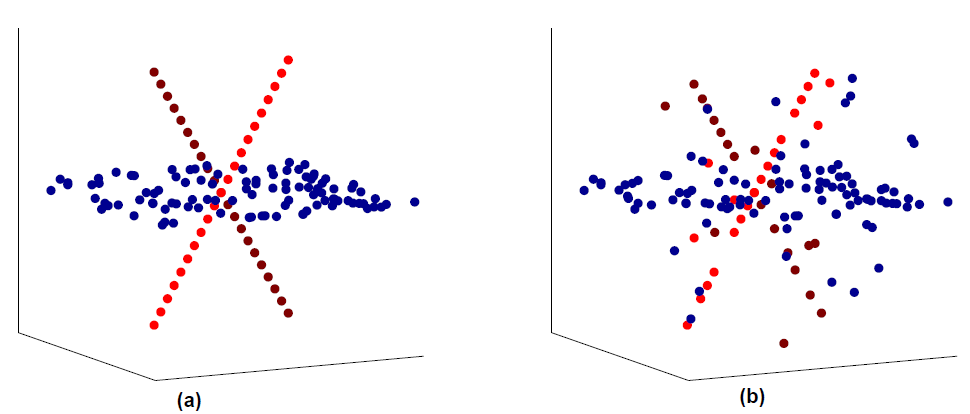
\includegraphics[width=0.8\linewidth]{Union_of_Subspace}
  \caption{采样于三个子空间的无噪音 (a) 和有噪音 (b) 数据}\label{fig:Union_of_sub_model}
\end{figure}
\begin{definition}[子空间聚类(Subspace clustering, SC)]\label{def:sc}
  有\(n\)个\(\R^d\)中的数据点\(x_i = y_i+z_i, \, i \in [n]\),
  \(y_i\)代表无噪音的理想点, \(z_i\)为噪音, \(y_i\)属于\(L\)个子空间的并
  \[\cS_1 \cup \cS_2 \cup\cdots\cup \cS_L,\]
  每个子空间\(\cS_\ell \subset \R^d\)的维度为\(d_{\ell} < d\),
  包含 \(n_{\ell}\)个数据点, 因此\(\sum_{\ell=1}^L n_\ell=n\). 
  子空间聚类是指将\(x_1, x_2, \ldots, x_n\) 分割为\(L\)类,
  使每一类对应一个子空间(注意, 下面为了表示方便, 通常把\(x_i, y_i, z_i\)
  按照列并在一起写成矩阵\(X, Y, Z\in \R^{d\times n}\)).
\end{definition}
\section{方法综述}
过去十年,子空间聚类问题引起广泛关注,人们提出了多种算法:
期望最大化(Expectation maximization)类型的局部优化算法,
比如 K-plane~\cite{bradley2000k} 和 Q-flat~\cite{tseng2000nearest};
代数方法,比如广义主成分分析(Generalized principal component analysis)~\cite{vidal2005generalized};
矩阵分解方法~\cite{costeira1995multi,costeira1998multibody}; 基于谱聚类的方法
~\cite{chen2009spectral,lauer2009spectral}; 自底向上的局部采样方法~\cite{rao2008motion,yan2006general};
以及基于自表示的方法,比如稀疏子空间聚类(Sparse subspace clustering, SSC)~\cite{elhamifar2009sparse,elhamifar2013sparse}
和低秩表示 (Low rank representation, LRR)~\cite{liu2010robust,liu2013robust}.
以上算法综述详见~\cite{vidal2010tutorial} 及其参考文献,
本文主要介绍SSC及其各种衍生算法.

\subsection{SSC和LRR}
2009年Elhamifar等首先将稀疏表示(Sparse representation)用于子空间聚类~\cite{elhamifar2009sparse}, 
提出基于自表示的SSC方法, 并在2013年加以完善~\cite{elhamifar2013sparse}, 使其成为目前公认表现最好的子空间聚类算法之一.
自表示的基本思想是: 因为数据点\(x_i\)的和另外一些点都在同一低维子空间中, 那么 
我们可以用其它点的线性组合表示\(x_i\), 即
\begin{equation}
  x_i \approx \sum_{i\neq j} [c]_j x_j, 
  \label{eq:rep}
\end{equation}
其中系数向量\(c\in \R^n, [c]_i = 0\). 
由于噪音干扰, 完全精确的表示不一定存在, 所以这里用了约等于.
如果数据点按列排成矩阵 \eqref{eq:rep} 等价于
\begin{equation}
  X \approx XC \quad \text{s.t.}\quad \diag(C) = \mathbf{0},
  \label{eq:matrix_rep}
\end{equation}
其中\(C\in \R^{n\times n}\), \(\diag(\cdot)\)是矩阵的对角线向量组成的对角阵.
利用表示矩阵\(C\)可以构造邻接矩阵\(W=(|C|+|C^T|)/2\),
这样子空间聚类问题就转化成\(n\)个点的无向图
分割问题, 我们可以谱聚类算法~\cite{ng2002spectral} 解决.

显然能否得到较好的表示系数是自表示方法成败的关键.
对于 \eqref{eq:rep} 我们希望表示系数\(c\)满足
\begin{equation}\label{eq:self_rep_1}
  [c]_j = 0, \quad  \forall j\in [n], \,y_j \notin \cS_\ell .
\end{equation}
即只用和\(x_i\)属于同一子空间的点表示\(x_i\).
这样的\(c\)必然比较稀疏(大部分位置都是零), 
于是SSC对无噪音和有噪音的数据分别求解 \eqref{eq:SSC} 和 \eqref{eq:ssc_noise}.  
\begin{gather}
  \min_{c} \; \|c\|_1\quad \text{s.t.}\quad y_i=Yc, \quad [c]_i=0 \label{eq:SSC}\\
  \min_{c} \; \|c\|_1+\frac{\lambda}{2}\left\|x_i-Xc\right\|_2^2, \quad \text{s.t.} \quad
  [c]_i = 0. \label{eq:ssc_noise}
\end{gather}
SSC利用\(\ell_1\)正则化迫使每个点只用较少的其它点表示,
这样所用点就很可能和\(x_i\)来自同一子空间.
\([c]_i = 0\)的约束是为了避免平凡解,
即每个数据仅用它自己表示自己.
Elhamifar等证明了在无噪音且子空间\(\cS_1, \cS_2, \ldots, \cS_L\)
相互独立(子空间只在原点相交)的情况下,
 \eqref{eq:SSC} 的解\(c\)满足 \eqref{eq:self_rep_1} ~\cite{elhamifar2013sparse}.
Cand\`{e}s等证明了带噪音半随机模型下, 当点和子空间分布满足一定条件时,
\(c\)有较大概率满足 \eqref{eq:self_rep_1} ~\cite{soltanolkotabi2014robust} .
把 \eqref{eq:ssc_noise} 写成矩阵的形式
\begin{equation}
  \begin{gathered}
    \min_C \; \|C\|_1+\frac{\lambda}{2}\left\|X-XC\right\|_F^2\\
    \text{s.t.} \quad \diag(C)=\mathbf{0}.
  \end{gathered}
  \label{eq:ssc_matrix}
\end{equation}
我们可以得到\autoref{alg:ssc}.  

\begin{algorithm}[tb]
  \caption{稀疏子空间聚类(Sparse subspace clustering)}
  \label{alg:ssc}
  \begin{algorithmic}
    \State {\bfseries 输入:}
    数据点组成的矩阵 \(X\in \mathbb{R}^{d\times
    n}\),类数\(L\)和正则化参数\(\lambda\)
    \State{1. } 求解 \eqref{eq:ssc_matrix},   得到最优解\(C\)
    \State{2. } 令 \(W=(|C|+|C|^T)/2\) 构造邻接图\(G\),其邻接矩阵为\(W\)
    \State{3. } 对 \(G\) 进行谱聚类 
    \State {\bfseries 输出:} 聚类结果
  \end{algorithmic}
\end{algorithm}

SSC只是单独考虑每个数据的稀疏表示, 缺少对
数据集全局结构的描述. 为反映数据集的全局结构,
2010年, Liu等提出基于低秩表示的子空间聚类方法LRR~\cite{liu2010robust} .
类似于SSC, LRR也是求解数据点的表示,
不过将\(\ell_1\)正则化换成了低秩,
\begin{equation}
  \min_{C} \; \rank(C)+\frac{\lambda}{2}\|X-XC\|_F^2. \label{eq:lrr}
\end{equation}
不过 \eqref{eq:lrr} 很难求解, 常用的办法是将\(\rank(C)\)松弛成\(\|C\|_*\),
\(\|\cdot\|_*\)是矩阵核范数,即矩阵奇异值之和.
这样 \eqref{eq:lrr} 变成一个凸优化问题. 再类似SSC,用解出的\(C\),构造
邻接矩阵\(W\), 最后谱聚类.

SSC和LRR在实际测试集上都有不错的表现.
例如在运动分割领域的Hopkins155测试集~\cite{tron2007benchmark}上,
他们都有很高的正确率~\cite{elhamifar2013sparse, liu2013robust}.
不过当类别增多时, SSC较LRR更优秀~\cite{elhamifar2013sparse}.

\subsection{其它自表示方法}
基于SSC和LRR产生了很多拓展和变形.
Wang等同时考虑低秩和稀疏性,得出了下面的优化问题~\cite{wang2013provable}
\begin{equation}\label{eq:scc_lrr}
  \begin{gathered}
    \min_{C} \; \|C\|_*+\mu \|C\|_1+\frac{\lambda}{2}\|X-XC\|^2 \\
    \text{s.t.}\quad \diag(C) = \mathbf{0}.
  \end{gathered}
\end{equation}
其中\(\mu,\lambda\)均为给定参数. 
Zhuang等在 \eqref{eq:scc_lrr} 的基础上加上系数矩阵\(C\)非负
的限制,以应用于半监督学习~\cite{zhuang2012non}.

SSC,LRR需要假定数据充足, 对样本不足的情形, Patel等
提出了隐式SSC (Latent SSC) 和隐式LRR(Latent LRR)模型~\cite{patel2015latent},
\begin{equation}
  \begin{gathered}
    \min_{P,C} \mathcal{J}_1(C)+\mathcal{J}_2(P, C, X) \\
    \text{s.t.}\quad PP^T=I, \diag(C)=\mathbf{0},
  \end{gathered}
  \label{eq:latent}
\end{equation}
其中\(\mathcal{J}_2=\lambda_1\|PX-PCX\|_F^2+\lambda_2\|X-P^TP
X\|_F^2,\)而\(\mathcal{J}_1(C)\)可以是\(\|C\|_1\)也可以是\(\|C\|_*\),
矩阵\(P\)可以看成是从原始数据空间到隐式空间线性变换,要求它的每一行
正交且模长为1. 虽然 \eqref{eq:latent} 是非凸的,但是数值实验表明
收敛到局部极小值只需要几步迭代.

为了进一步提高子空间聚类的精度, Lu使用了Trace LASSO改进SSC,
提出相关自适应子空间分割 (Correlation adaptive subspace
segmentation, CASS)~\cite{lu2013correlation}, 
对每个数据点\(x_i\)求解
\begin{equation}
  \min_{c}\, \|X\diag(c)\|_* + \frac{\lambda}{2}\|x_i - Xc\|_2^2,
  \label{eq:cass}
\end{equation}
其中\(\diag(c)\)是以\(c\)为对角线的矩阵.如果把\(X\)的每一列按照\(\ell_2\)范数
归一化,Trace LASSO具有插值性质:
\[
  \|c\|_2\le \|X\diag(c)\|_*\le \|c\|_1.
\]
左端等式在数据是完全相关时(每列方向相同或相反)达到,右端在数据是完全无关时(列之
间正交)达到,这使得Trace LASSO能自适应数据的相关性.

Cand\`{e}s等指出在原有的\(\ell_1\)正则化参数上加上
适当权重, 可以进一步提高稀疏度~\cite{candes2008enhancing}.
于是Pham等提出了加权SSC (Weighted SSC)~\cite{pham2012improved},即求解下面的优化问题
\begin{equation}
  \begin{gathered}
    \min_{C}\, \|W\odot C\|_1 + \frac{\lambda}{2}\|X-XC\|_F^2 \\
    \quad \text{s.t.}\quad \diag(C) = \mathbf{0},
  \end{gathered}
  \label{eq:wssc}
\end{equation}
其中\(W\)是某个权重矩阵,比如可以取
\[
  W_{i,j} = \left( \exp\left\{ -\frac{\|x_i-x_j\|_2}{\mu}
\right\} \right)^{-1},
\]
其中\(\mu\)是给定参数.由于实际应用中空间距离近的点是同类的概率较大,
上面的权重矩阵可以使自表示时更倾向于用附近的点,从而提高准确率.

如果SSC或者LRR产生的邻接矩阵是严格块对角的, 那么谱聚类的效果
很可能较好,所以Feng等提出块对角稀疏子空间聚类
(Block-diagonal sparse subspace clustering, BD-SSC)模型~\cite{feng2014robust}.
在优化 \eqref{eq:ssc_noise} 和 \eqref{eq:lrr} 时, BD-SSC加上了\(C \in \cK\) 的限制,其中
\[
  \cK = \left\{ \rank(L_W)=n-L, W=\half\left( |C|+|C^T| \right) \right\},
\]
\(L\)是子空间类数,\(L_W=\diag(W)-W\).
在寻找表示矩阵\(C\)时, BD-SSC预先要求其有比较好的可分性, 从而提高谱聚类正确率. 
不过如此一来优化问题高度非凸, 虽然可以用交替方向投影方法求解, 但是结果比较依赖初始值选取.

Yuan等首先引入组稀疏范数, 提出了稀疏生成子空间聚类
(Sparse additive subspace clustering, SASC)~\cite{yuan2014sparse}.
其想法是: 虽然同类的数据点理论上在一个线性子空间中,
但由于噪音干扰可能失去了线性性, 因此直接做线性回归无法取得好的效果,
如果我们用一族变换\(\left\{T_1, T_2, \cdots, T_m\right\}\)作用到每个点\(x_i\)上,
可以生成\(m\)个新的数据点\(\left\{ T_1 x_i, T_2 x_i,\cdots,
T_m x_i \right\}\),其中很可能包含比\(x_i\)更接近无噪音的点. 
我们把每个原始的数据点\(x_i\)相对于\(n\times m\)个新生成的
数据点做回归,由于新数据天然具有组别(同一点生成的自然是一组),
令代表组别信息的指标集族
\begin{equation*}
  \Omega:= \left\{ \{1,\ldots, m\}, \{m+1, \ldots, 2m\}, \ldots, \{(n-1)m+1,
  \ldots, nm\}\right\}.
\end{equation*}
对每个\(x_i\)求解
\begin{equation}
  \begin{gathered}
    \min_{c}\, \|c_i\|_{\Omega, 1}+\frac{\lambda}{2}\|x_i-\left[ 
      T_1 x_1, \cdots, T_m x_1,\cdots, T_1 x_n, \cdots, T_m x_n
    \right] c\|_2^2 \\
    \text{s.t.} \quad [c]_j = 0,\,\, (i-1)m < j \le i\cdot m,
  \end{gathered}
  \label{eq:sasc}
\end{equation}
其中\(\|c\|_{\Omega, 1}\)范数是将向量的分量\(m\)个一组,每组的\(\ell_2\)范数加和.
SASC在变换选取适当时,有很好的表现,但是变换选取的不确定性是其重要缺陷.

\chapter{多任务和组稀疏方法}\label{chp:prob_setup}
本章我们具体地介绍受SSC启发的新算法.

虽然SSC是目前最优秀的子空间聚类算法之一,但是它有两个缺陷:第
一,SSC 每次只考虑一个点相对于其它点的表示,
这比较容易受到噪音和异常点的干扰. 如果我们预先知道点\(x_1, x_2, x_3\)
属于同一类,然后寻找其他能同时表示\(x_1, x_2, x_3\)的点, 这无疑比
单独考虑\(x_1\)或\(x_2\)或\(x_3\)更稳健. 第二, 在SSC 模型中,
我们要求表示尽量稀疏, 然而过分稀疏的邻接矩阵, 可能在
接下来的谱聚类中没有比较好的可分性. 事实上最优的邻接图应该是
同一子空间上的点之间连接尽量多,不同子空间的点之间连接尽量少.
如果我们能让表示向量既不对应不同子空间的点又不集中在
少数几个点上,这样产生的邻接图聚类效果很可能更好.

基于上面的考虑,本文结合压缩感知中的联合稀疏(joint sparse) 模型\cite{yuan2012visual},
提出了新的子空间聚类方法,它的核心内容分两步:
第一步是根据点的空间信息,先将某些点聚在一起,组成若干组.
第二步是求解自表示系数, 有两种方法:
可以把一组点作为整体,相对其他点做回归,要求他们被同时表示,
这是\emph{多任务稀疏子空间聚类}
(Multi-task Sparse Subspace Clustering, MT-SSC). 也可以依然像SSC那样,
将一个点用其他点表示,但是采用组稀疏的优化范数,
得到\emph{组稀疏子空间聚类}(Group Sparse Subspace Clustering, G-SSC).
两种方法都可以得到表示系数,进而构造邻接矩阵, 最后谱聚类

\section{分组算法} 
第一步要将数据点分成若干组,尽量使每一组里的点属于同一个子空间.
为了做到这点最直接的想法是用\(K\)近邻算法, 将每个点和它的邻居分为一组.
然而如果只考虑数据点之间的欧式距离, 无疑忽略了线性空间的性质.
所以我们类似于~\cite{heckel2013noisy}, 用两点之间的夹角作为距离度量,即
\[d(x_i,x_j)=\exp\left\{-\cos^{-1}\left( \frac{|\langle x_i,
x_j\rangle|}{\|x_i\|_2\|x_j\|_2} \right)\right\}.\]
不过如果单纯考虑夹角,也只能利用一个维度上的信息, 我们更近一步地定义
点到点集的投影距离
\[ d(a, A, r) =  \|a\|_2-\|U^Ta\|_2 \]
其中\(a \in R^d\)代表一个数据点,\(A\in \R^{d\times m}\)是一组数据点组成的矩阵,
\(r\)为正整数, \(U\)是对\(A\)做奇异值分解后的前\(\min(r, \rank(A))\)个左奇异向量组成的矩阵.
\(r\)的大小可以
事先给定,也可以取\(A\)的有效秩\cite{yan2006general}
\[
  r = \argmin_{\tldr} \frac{\sigma_{\tldr+1}^2}{\sum_{i=1}^{\tldr}
  \sigma_{\tldr}^2} +\kappa \tldr,
\]
其中\(\sigma_1,\sigma_2,\cdots,\sigma_m\)是\(A\)的奇异值,\(\kappa\)是和噪音大小有关的参数.

我们从一个点\(x_0\)出发, 在没有什么信息的情况下, 自然取\(k\)个夹角最近邻
\(x_1, x_2, \ldots, x_k \)为一组,于是邻居集合
\(\cN := \left\{ x_0, x_1, \ldots, x_k \right\}.\)
接着用这\(k+1\)个点张成\(r\)维平面, 我们得到投影矩阵\(U\),再取\(k\)个投影最近邻,更新\(\cN\)和
\(U\),如此循环, 退出条件是最大相对误差大于阈值\(\theta\),即
\[\max_{x\in \cN} \frac{\|x\|_2-\|U^T x\|_2}{\|x\|_2} > \theta.\]
于是我们得到计算每个点的拓展最近邻的\autoref{alg:nsn}.
\begin{algorithm}[tb] \caption{拓展最近邻}\label{alg:nsn}
  \begin{algorithmic}
    \State \textbf{输入:} \(n\) 个数据点 \(\cX = \{x_1,\ldots,x_n\}\),
    \(\cX\)中的某个数据点\(x_0\), 邻居增长数\(k\),子空间维度\(r\)(或有效秩参数\(\kappa\)),噪音控制参数\(\theta\).
    \State 初始化:将所有向量归一化,\(U = x_0, \cX = \cX \setminus x_0,
    \cN=\{x_0\}\) 
    \Repeat
    \State{1. } 对每个\(x\in \cX\)计算\(\|U^Tx\|_2\),取出前\(k\)大的点组成集合\(\cN_0\)
    \State{2. } \(\cX = \cX \setminus \cN_0, \cN = \cN \cup \cN_0\)
    \State{3. } \(U\)取为\(\cN\)中所有点组成的矩阵做奇异值分解的前\(r\)个左奇异向量
    (或取\(r\)为\(\cN\)中点组成矩阵的有效秩)
    \State{4. } \(\text{err}=1 - \min_{x \in \cN}\|U^T x\|_2\)
    \Until{\(\text{err}>\theta\)}
    \State \textbf{输出:} \(x_0\)的拓展最邻居集合\(\cN \setminus \cN_0\)
    \Comment{有可能只有\(x_0\)自身}
  \end{algorithmic}
\end{algorithm}

由于我们引入了阈值\(\theta\), 使得\autoref{alg:nsn} 有一定的自我修正能力.
如果参数\(k\)取得过大, 或者循环进行多步后, 很可能会在邻居集合\(\cN\)
中混入其他子空间的点, 这时\(\cN\)中的点就不能很好地分布在一个\(r\)维平面上,
使得\(\text{err}>\theta\), 然后我们会从\(\cN\)中删去所有上一步加入的点, 这样
混入的错误点又会被剔除. 

得到每个点的近邻之后,还要把点分成若干组,因为这些近邻之间有重叠, 但是后面的MT-SSC
和G-SSC要求每个点只能在一个组中. 当然这里可以使用谱聚类等聚类算法, 不过简单
起见,我们直接采用``先到先得''的原则:先找到一个未分组的点\(x_0\).
将其近邻集合\(\cN(x_0)\)中没有分组的和它分成一组,再找下一个未分组点,直到分完所有点.
注意每个点都一定和它邻居集合的子集在一组, 所以如果邻居集合没有包含错误点, 那么分组
也一定没有错误, 如果邻居集合包含错误点, 也可能会得到正确的分组,
因为邻居集合有重叠.
实际计算中,为了消除取点带来的随机性,我们总是按照点的\(\ell_2\)范数从大到小,依次选取.
对于每个分组, 我们将其所含点的编号组成一个指标集\(\cI \subset [n]\),
于是分组算法最终可以给出一个指标集族\(\Omega\), 满足
\begin{gather}
  \cI_i \cap \cI_j = \emptyset,\quad \forall \,\cI_i, \cI_j \in \Omega\quad \cI_i
  \neq \cI_j, \label{eq:nointer}\\
  \bigcup_{\cI\in \Omega} \cI = [n].\label{eq:full} 
\end{gather}
这保证了\(\Omega\)是对所有数据点的一个剖分, 从而有后面的多任务和组稀疏方法.

\section{多任务和组稀疏方法}
先介绍一些记号: 我们用\(X_i\) 表示矩阵\(X\) 的第\(i\)列,
\(X_{(i)}\)表示矩阵\(X\)的第\(i\)行,
\(X_{i,j}\)表示矩阵的第\(i\)行第\(j\)列的元素.
对某个指标集\(\cI\subset [n]\), \(\cI^c:=[n]\setminus \cI\).
\(x_\cI\)表示向量\(x\)中对应指标集\(\cI\)的部分,
\(X_\cI\)表示将矩阵\(X\)的列向量按照指标集\(\cI\)取出后组成的子矩阵, 
\(X_{(\cI)}\)表示将矩阵\(X\)的行向量按照指标集\(\cI\)取出后组成的子矩阵,
\(X_{\cI, \cJ}\)表示行按指标集\(\cI\)抽出, 列按指标集\(\cJ\)抽出组成的子矩阵. 
给定满足\eqref{eq:nointer}\eqref{eq:full}的指标集族\(\Omega\),
定义向量范数\(\|x\|_{\Omega, 1}:=\sum_{\cI \in \Omega} \|x_{\cI}\|_2\),
矩阵范数\(\|X\|_{\Omega, 1}:=\sum_{i} \|X_i\|_{\Omega, 1}\).
再定义矩阵范数\(\|X\|_{2, 1}:=\sum_{i} \|X_i\|_2\).

\subsection{MT-SSC}

SSC对每个点\(x_i\)求解\eqref{eq:ssc_noise},
而有了指标集族\(\Omega\)后, 对于\(\cI\in \Omega\),
可以得到多列数据组成的矩阵\(X_\cI\), 我们希望找到一些点能同时表示
\(X_\cI\)的每一列, 即考虑下面的优化问题
\begin{equation}\label{eq:multi}
  \begin{gathered}
    \min_{C}\; \|C^T\|_{2, 1} + \frac{\lambda}{2} \|X_\cI - XC\|_F^2\\
    \text{s.t.} \quad C_{(\cI)} = \mathbf{0},
  \end{gathered}
\end{equation}
\(C \in \R^{n \times |\cI|}\)是点集\(\{x_i, \forall\, i\in \cI\}\)的表示矩阵,
\(\ell_{2,1}\)范数的正则化项能使 \(C\)在非零行向量较少, 而非零行向量对应的点
能同时表示\(X_\cI\)的每一列, 约束条件是为了排除自己表示自己这种平凡情形.
如果我们所有分组一起考虑, 把\eqref{eq:multi}改写成
\begin{equation}\label{eq:multi_matrix}
  \begin{gathered}
    \min_C\; \|C^T\|_{\Omega, 1} + \frac{\lambda}{2} \|X-XC\|_F^2 \\
    \text{s.t.} \quad C_{\cI, \cI} = \mathbf{0}, \quad \forall \, \cI \in
    \Omega,
  \end{gathered}
\end{equation}
其中\(\|\cdot\|_{\Omega, 1}\)为矩阵每列的\(\ell_{\Omega, 1}\)范数加和.
我们要用\eqref{eq:multi_matrix}的解\(C\)组成邻接矩阵\((|C|+|C^T|)/2\),
进而做谱聚类. 不过不同于SSC, 我们在每个分组内部缺少邻接关系,
因此对\(i, j\in\cI\) 取\(C_{i, j} = \max(|C_\cI|)\), 这样就能构造出完整的邻接矩阵.
MT-SSC同时考虑多个点的回归, 所以应该会比SSC更加稳健, 同时注意到\eqref{eq:multi}
的解在非零行上应该是稠密的, 则其生成的邻接图在同一子空间内部的连接会更紧密.

\subsection{G-SSC}
不同于\eqref{eq:ssc_noise}, G-SSC对每个\(x_i\)考虑下面的优化问题
\begin{equation}
  \begin{gathered}
    \min_{c} \; \|c\|_{\Omega, 1} + \frac{\lambda}{2} \|x_i - Xc\|_2^2\\
    \text{s.t.} \quad [c]_i = 0.
  \end{gathered}
  \label{eq:group}
\end{equation}
其中\(\cI\)是\(\Omega\)中包含\(i\)的指标集, 由\eqref{eq:nointer}和\eqref{eq:full}
可知\(\cI\)存在且唯一. \eqref{eq:group}相当于用某些组的点来表示\(x_i\), 相比于
独立考虑每个点, 这样能减少异常点的干扰, 也能使得到的表示矩阵相对稠密.
同样地,写出\eqref{eq:group}的矩阵形式
\begin{equation}
  \begin{gathered}
    \min_C\; \|C\|_{\Omega, 1} + \frac{\lambda}{2} \|X-XC\|_F^2 \\
    \text{s.t.} \quad \diag(C) = \mathbf{0}.
  \end{gathered}
  \label{eq:group_matrix}
\end{equation}
用\eqref{eq:group_matrix}的解\(C\)组成邻接矩阵\((|C|+|C^T|)/2\), 进而做谱聚类.

注意如果\autoref{alg:nsn} 的参数\(\theta\)取得很小, 那么每个点的最近邻集合
将只包含自己, 于是MT-SSC和G-SSC将退化成SSC, 所以如果参数选取适当, MT-SSC
和G-SSC的聚类结果至少不会比SSC差.

\subsection{ADMM算法}
下面讨论如何求解MT-SSC和G-SSC的优化问题.
\eqref{eq:multi_matrix} 和 \eqref{eq:group_matrix} 可以写成统一的形式
\begin{equation}\label{eq:MatrixLasso}
  \begin{gathered}
    \min_{C} \; \|C\|_{\Omega}+\frac{\lambda}{2}\|X-XC\|_F^2  \\
    \text{s.t.} \quad \Bdiag(C)=\mathbf{0},
  \end{gathered}
\end{equation}
其中\(\|\cdot\|_{\Omega}\) 为某个与指标集族\(\Omega\)有关的凸范数,
对于MT-SSC, \(\|C\|_{\Omega}=\|C^T\|_{\Omega, 1}\), 
\[
  \Bdiag(C)=\begin{bmatrix}
    C_{\cJ_1, \cJ_1}  & \mathbf{0} & \cdots & \mathbf{0} \\
    \mathbf{0}  & C_{\cJ_2, \cJ_2} & \cdots & \mathbf{0} \\
    \vdots   &    \vdots    &    \ddots     & \vdots \\
    \mathbf{0}  &  \mathbf{0} &  \cdots  & C_{\cJ_{|\Omega|},\cJ_{|\Omega|}}
  \end{bmatrix}
\]
其中\(\{\cJ_1, \cJ_2,\ldots,\cJ_{|\Omega|}\}=\Omega\),
对于G-SSC, \(\|C\|_{\Omega}=\|C\|_{\Omega, 1}, \Bdiag(C) = \diag(C)\).

我们用ADMM算法~\cite{stephen2011distributed} 求解\eqref{eq:MatrixLasso}
如果适当交换\(X\)列向量的顺序, 将同一组的点排在一起, 
那么\eqref{eq:MatrixLasso}可以写成下面的等价形式
\begin{equation}\label{eq:MatrixLasso_modify}
  \begin{gathered}
    \min_{C} \; \|C\|_{\Omega}+\frac{\lambda}{2}\|X-XJ\|_F^2 \\
    \text{s.t.} \quad J=C-\Bdiag(C).
  \end{gathered}
\end{equation}
我们写出\eqref{eq:MatrixLasso_modify}的Lagrangian,并在其上增加一个等价
的二次惩罚项得到增广Lagrangian
\begin{multline*}
  \cL= \|C\|_{\Omega}+\frac{\lambda}{2}\|X-XJ\|_F^2 
  +\frac{\mu}{2}\|J-C+\Bdiag(C)\|_F^2\\
  +tr(\Lambda^T(J-C+\Bdiag(C))),
\end{multline*}
其中\(\Lambda\)是对偶变量,\(\mu\)是给定参数.为了交替优化
\(J\), \(C\) 和 \(\Lambda\) 直到收敛,需要求解 \(\partial \cL/\partial J=0\)
和 \(\partial \cL/\partial C=0\). 由\(\partial \cL/\partial J=0\) 可得
\[
  J=(\lambda X^TX+\mu I)^{-1}\left(\lambda X^TX+\mu C - 
  \mu\Bdiag(C)-\Lambda\right).
\]
另一方面, 虽然\(\cL\)关于\(C\)不可导, 但极值可以用拓展的
Soft-Threshold 算子~\cite{donoho1995noising}求得.
先定义
\begin{equation*}
  S_\alpha(a) = \begin{cases}
    \mathbf{0} & \|a\|_2 \le \alpha, \\
    (\|a\|_2 - \alpha) \frac{a}{\|a\|_2} & \|a\|_2 > \alpha.
  \end{cases}
\end{equation*}
其中\(\alpha\)为给定正数,\(a\)为任意向量.
再定义\(\sfth_{\alpha,\Omega}:\R^n\rightarrow \R^n\), 若
\(b =\sfth_{\alpha,\Omega}(a)\), 则\( b_\cI= S_\alpha(a_\cI),
\, \forall \cI \in \Omega\).

\begin{algorithm}[tb]
  \caption{求解MT-SSC和G-SSC的优化问题}
  \label{alg:MatrixSSC}
  \begin{algorithmic}
    \State {\bfseries 输入:}
    \(n\) 个样本点 \(x_1,\ldots,x_n\),它们组成了数据矩阵\(X\in \R^{d\times
    n}\),组别信息\(\Omega\),参数\(\lambda\) 和 \(\mu\)
    \State 初始化 \(C=0\), \(J=0\), \(\Lambda=0\)
    \While{未收敛}
    \State{1. } 更新 \(J\) 
    \[J=(\lambda X^TX+\mu I)^{-1}(\lambda X^TX+\mu C-\Lambda).\]
    \State{2. } 更新 \(C\)
    \[ C^{'}=\sfth_{\frac{1}{\mu},\Omega}\left(J+\Lambda/\mu\right), \]
    \[ C=C^{'}-\Bdiag(C^{'}).\]
    \State{3. } 更新 \(\Lambda\)
    \[\Lambda=\Lambda+\mu(J-C)\]
    \EndWhile
    \State 对MT-SSC要取每组的绝对值最大值将\(C\)补充完整
    \State {\bfseries 输出:} 最优解\(C\)
  \end{algorithmic}
\end{algorithm}
求解\eqref{eq:multi_matrix}时, 我们将\(\sfth\)作用在矩阵
\(J+\Lambda/\mu\)的每一个行向量上,
求解\eqref{eq:group_matrix}时作用于列向量,
最终得到\autoref{alg:MatrixSSC}.
注意到 \((\lambda X^TX+\mu I)^{-1}\)
能被预先算好,这样每次迭代的时间就主要花在计算矩阵乘法上,
因此MT-SSC,G-SSC花在优化上的时间和SSC几乎相同.

下面我们给出拓展最近邻算法,MT-SSC和G-SSC的一些理论分析,以及数值实验结果.

\chapter{算法的理论分析}\label{chp:theory}
本章将给出拓展最近邻算法, MT-SSC和G-SSC的理论分析, 尝试考察在什么条件算法能
给出较好结果. 对拓展最近邻算法而言, 理想的结果是每个邻居集合中的点都属于同一个子空间;
对MT-SSC和G-SSC而言, 理想的结果是生成的邻接图没有错误连接, 也就是
每个点只用了和自身同一子空间的点表示. 算法正确与否和子空间之间的夹角, 
数据点的分布, 噪音大小都有关系, 所以我们先定义出一些度量各种关系的量,
然后证明当这些量满足一定条件时算法能够保证正确. 先介绍本章的记号和基本假设.

\section{记号与模型}
先介绍一些本章将用到的记号:
对矩阵\(X\in\R^{d\times n}\)和指标集\(\cI \subset [n]\)
我们用\(X_{\cI\rightarrow 0}\)表示将\(\cI\)对应的列置为零后的矩阵,
如
\[
  X_{\{i\}\rightarrow 0} = \left[ X_1, X_2, \cdots, X_{i-1}, \mathbf{0},
  X_{i+1}, \cdots, X_n \right].
\]
令指标集\(\cI_\ell\)表示子空间\(\cS_\ell\)包含点的编号,
即\(y_i\in \cS_\ell, \forall i\in \cI_\ell\).
简记\(X_\cI^{(\ell)}:=X_{\cI\cap\cI_\ell}, X_{\cI^c}^{(\ell)}:=X_{\cI^c\cap \cI_\ell}\),
同理\(Y_\cI^{(\ell)}:=Y_{\cI\cap \cI_\ell}, Y_{\cI^c}^{(\ell)}:=Y_{\cI^c\cap
\cI_\ell}\),
注意 \(\cI^c \cap \cI_\ell = \cI_\ell \setminus \cI\), 所以
\(X_{\cI^c}^{(\ell)} = X_{\cI_\ell \setminus \cI}\),
即表示取出子空间\(\cS_\ell\)中的点, 除非编号在\(\cI\)中.
花体字母 \(\cX\) 表示矩阵\(X\)的所有列向量组成的集合, \(\cX_\ell\)表示矩阵\(X_{\cI_\ell}\)
所有列向量组成的集合, 同理有\(\cY\)和\(\cY_\ell\).
用\(\cP(X)\) 表示矩阵\(X\)所有列向量张成的对称凸包,即
\(\cP(X) = \mathrm{conv}(\pm \cX)\).简记
\(\cP_{\cI^c}^{(\ell)} := \mathcal{P}(X_{\cI^c}^{(\ell)}),
\cQ_{\cI^c}^{(\ell)} :=\mathcal{P}(Y_{\cI^c}^{(\ell)})\).
\(\P_\cS\) 表示子空间\(\cS\) 的投影矩阵.

我们考虑两种不同的数据模型:\emph{确定性模型}和\emph{半随机模型}\cite[1.4.1]{soltanolkotabi2012geometric}.
在确定性模型中, 无噪音数据点和子空间都是任意给定的, 噪音大小受到控制.
而半随机模型假设每个无噪音数据点\(y_i\)在子空间\(\cS_\ell\)中独立均匀分布.
\autoref{sec:proof_greedy}的分析基于半随机模型,
\autoref{sec:proof_multi}和\autoref{sec:proof_group}基于确定性模型,
同时在本章中始终假设\(y_i\)是单位向量 (单位化的条件能使后面的证明叙述简洁,
只需要对条件稍作修改我们的结论就能拓展到一般情形).

\section{拓展最近邻的理论分析}\label{sec:proof_greedy}
在\autoref{alg:nsn} 中,每执行一次循环, 新加入的点都会影响投影平面,
导致理论分析比较困难,因此我们只能给出执行第一次循环,即\(U=x_0\)时
算法的正确性条件(每个点的拓展最近邻都和自身在同一子空间).

我们假设样本点满足\emph{半随机模型},即每个子空间是确定的,
但是数据点在每个子空间中随机生成的.进一步地,
由于数据点都是单位向量,因此它们独立均匀采样于各自子空间的单位球.
简单起见,我们假定每个子空间的维度和点数相同,即\(d_0:= d_1=\cdots=d_L,
n_0:= n_1=\cdots=n_L\),且不考虑噪音.

令\(D_i\in \R^{d\times d_0}, i\in [L]\)为子空间\(\cS_i\)的正交基组成的矩阵.两个
子空间的\emph{相似度}定义为
\begin{align*}
  \aff(i,j) := \frac{\|D_i^\top D_j\|_F}{\sqrt{d_0}} \in [0, 1].
\end{align*}
子空间 \(\cS_i\) 和 \(\cS_j\) 完全一样当且仅当 \(\aff(i,j) = 1\).
若 \(\aff(i,j) = 0\),那么 \(\cS_i\) 中的任意向量垂直于 \(\cS_j\).
我们定义最大相似度为
\[ \max \aff := \max_{i,j \in [L], i \neq j} \aff(i,j) \in [0,1].\]

根据以上假设,我们共有 \(n = n_0 L\) 个点,每个点 \(y_i\)(无噪音的数据点用\(y\)表示)
独立同分布地均匀采样于\(\S^{d-1} \cap \cS_{\ell_i}\) ,
\(\S^{d-1}\) 是 \(\R^d\) 中的单位球,\(\ell_i\)是\(y_i\)所属子空间的编号,于是
\[
  y_i = D_{\ell_i} w_i ,\quad w_i \sim \Unif(\S^{d_0-1}) ,\quad
  \forall i \in [N].
\]
相当于每个\(y_i\)都是由低维空间的\(w_i\)生成的.
我们要证明在某些条件下,对点\(y_i\),当\(U=y_i\)时,
它的\(k\)个投影最近邻有\emph{较大概率}和\(y_i\)在同一子空间中.
比如对于点\(y_1\),就要求
\begin{equation}
  |y_1^T y_k|>|y_1^T y_j| \quad \forall j \in \{j:\ell_j \ne \ell_1\},
  \label{eq:greedy_ineq}
\end{equation}
其中 \(y_k\) 为\(\ell_1\)类中在\(y_1\)上投影第\(k\)大的点.
因此我们要得到\eqref{eq:greedy_ineq}左边的下界和右边的上界.

\subsection{异类投影的上界}
我们希望和\(y_1\)不同子空间的点\(y_j\)在\(y_1\)上的投影
被子空间的最大相似度\(\maff\)控制.
由于\(|y_1^T y_j| = |w_1^T D_1^T D_j w_j|\), 而\(w_j \sim \Unif(\S^{d_0-1})\),
所以我们要考察随机变量\(\|D_j^T D_1 w_1\|_2\).

\begin{lemma} \label{lem:expectation}
  若 \(u \sim \Unif(\mathbb{S}^{d-1})\) 和任意矩阵 
  \(A \in \mathbb{R}^{m \times d}\),我们有
  \[ \E[\|Au\|_2^2] = \frac{1}{d} \|A\|_F^2. \]
\end{lemma}
\begin{proof}
令 \(A = U \Sigma V^T\) 为 \(A\) 的奇异值分解,于是
\begin{align*}
  \E[\|Au\|_2^2] &= \E[\|U \Sigma V^T u\|_2^2]= \E[\|\Sigma V^Tu\|_2^2] 
  = \E[\|\Sigma u\|_2^2]\\
  &= \sum_{i=1}^{\min(m,d)} \sigma_i^2 \E[ [u]_i^2] 
  = \sum_{i=1}^{\min(m,d)} \sigma_i^2 \cdot \frac{1}{d} = \frac{1}{d} \|A\|_F^2.
\end{align*}
因为\(V\)是正交阵, 所以\(u\sim V^T u\), 于是\(\E[\|\Sigma V^Tu\|_2^2]
=\E[\|\Sigma u\|_2^2]\). 而\(\E[[u]_i^2] = \frac{1}{d}\), 
是因为\(u\)的每个分量对称, 期望相同, 同时\(\sum_{i=1}^d \E[ [u]_i^2] = 1 \),
\end{proof}

下面介绍著名的L\'{e}vy引理\cite[页6]{ledoux2005concentration}.
\begin{lemma}\label{lem:measureconc}
  若 \(u \sim \Unif(\mathbb{S}^{d-1}), f:\S^{d-1}\rightarrow
  \R\),且Lipschitz连续,即
  \[|f(a)-f(b)|\le \eta\|a-b\|_2 \quad \forall\, a, b\in \S^{d-1},\]
  其中\(\eta\)是Lipschitz常数,于是
  \begin{align*} 
    \Pr \left\{f(u)  > M_f + \alpha \right\}&\le \exp \left(-
    \frac{d}{2} \cdot \frac{\alpha^2}{\eta^2} \right),\\
    \Pr \left\{f(u)  < M_f - \alpha\right\}&\le \exp \left(-
    \frac{d}{2} \cdot \frac{\alpha^2}{\eta^2} \right),
  \end{align*}
对任意\(\alpha > 0\)成立. 其中\(M_f\)是\(f(u)\)的中位数.
\end{lemma}
根据L\'{e}vy引理可得一个常用的推论.
\begin{corollary} \label{cor:mean_median}
  若 \(u \sim \Unif(\mathbb{S}^{d-1}), f:\S^{d-1}\rightarrow
  \R\),且Lipschitz连续,即
  \[|f(a)-f(b)|\le \eta\|a-b\|_2 \quad \forall a, b\in \S^{d-1},\]
  其中\(\eta\)是Lipschitz常数,我们有
  \begin{align}
    |\E[f(u)]-M_f|\le \sqrt{\frac{2\pi}{d}}\eta.
    \label{eq:mean_median}
  \end{align}
\end{corollary}
\begin{proof}
  由\autoref{lem:measureconc}可得
  \[\Pr\left\{|f(u)-M_f|>\alpha\right\} \le 2 \exp \left(
  -\frac{d}{2}\cdot \frac{\alpha^2}{\eta^2} \right).\]
  于是
  \begin{align*}
    |\E[f(u)]-M_f|\le& \E\left|f(u)-M_f\right|= 
    \int_0^\infty \Pr\left\{\left|f(u)-M_f\right|>\alpha \right\}\mathrm{d}\alpha\\
    \le& 2 \int_0^\infty \exp\left( 
    -\frac{d}{2}\cdot \frac{\alpha^2}{\eta^2} \right)\mathrm{d}\alpha =
    \sqrt{\frac{2\pi}{d}}\eta.
  \end{align*}
  上式中的第一个等号由Fubini定理保证.
\end{proof}
若令\(A:=D_j^T D_1, f(w_1):=\|D_j^T D_1 w_1\|_2, w_1\sim \Unif(\S^{d_0})\),
我们希望\(\|A w_1\|_2\le c(\maff)\)有较大概率成立,
\(c(\maff)\)是依赖\(\maff\)的某个常数.
由\autoref{lem:expectation}可知\(\|A w_1\|_2\)的期望与\(\|A\|_F\)有关,
而\(\|A\|_F=\|D_1^T D_j\|_F\)被\(\maff\)控制.
于是我们结合\autoref{lem:measureconc} 和\autoref{cor:mean_median}
得到\autoref{lem:upper}.
\begin{lemma} \label{lem:upper}
  对\(u \sim \Unif(\S^{d-1})\)和任意矩阵\(A\in \R^{m\times d}\),则
  \[
    \Pr \left\{ \| Au \|_2  \le \frac{\|A\|_F}{\sqrt{d}} +
    \left (\sqrt{\frac{2\pi}{d}}+\delta\right )\|A\|_2\right\} > 1- \exp \left(
    -\frac{d}{2} \delta^2 \right),
  \]
  对任意\(\delta>0\)成立
\end{lemma}
\begin{proof}
  令\(f(u):=\|Au\|_2\),则\(f(u)\) Lipschitz连续,其Lipschitz常数为\(\eta:=\|A\|_2\),
  于是对任意\(\delta>0\)有
  \begin{align*}
    \Pr \left\{ f(u) > \frac{\|A\|_F}{\sqrt{d}} + 
    \left (\sqrt{\frac{2\pi}{d}}+\delta\right)\eta\right\} &=
    \Pr \left\{ f(u) > \sqrt{\E[f^2(u)]}+
    \sqrt{\frac{2\pi}{d}}\eta+\delta\eta\right\} \\
    &\le \Pr \left\{ f(u) > \E[f(u)] +
    \sqrt{\frac{2\pi}{d}}\eta+\delta\eta\right\} \\
    &\le \Pr \left\{ f(u) > M_f+\delta\eta \right\}\\
    &\le \exp\left( -\frac{d}{2}\delta^2 \right).
  \end{align*}
  第一个等号由\autoref{lem:expectation}, \(\E[f^2(u)]= \|A\|_F^2/d\),
  第一个不等号是由Jensen不等式, \(\E[f^2(u)]\ge (\E[f(u)])^2\),
  第二个不等号由\autoref{cor:mean_median},第三个不等号由\autoref{lem:measureconc},
  取\(\alpha=\delta\eta\). 最后再取互补事件即可.
\end{proof}

\subsection{同类投影的下界}
对于与\(y_1\)同类的点我们要考察第\(k\)大投影值的下界.
\begin{lemma}[\cite{ball1997elementary}引理~2.2,2.3]\label{lem:spherical_cap}
  对 \(u \sim \Unif(\S^{d-1})\) 和任意固定的向量 \(a\),我们有
  \begin{equation*}
    \left( \frac{1-\varepsilon}{2} \right)^{\frac{d-1}{2}} \le
    \Pr\left\{|a^Tu|>\epsilon \|a\|_2\right\} \le 2e^{\frac{-d\epsilon^2}{2}}
  \end{equation*}
\end{lemma}

\begin{lemma} \label{lem:projbound_lower}
  设 \(u_1, \ldots, u_n \) 为采样于\(\Unif(\S^{d-1})\) 的独立同分布随机向量,
  \(a \in \R^d \) 是固定向量,
  令 \(\alpha^{(k)}\) 为 \(\{\alpha_i:= |a^T u_i|, 1 \le i \le n\}\) 中的第\(k\)大值.
  若存在\(\delta > 0\), 满足
  \[\delta \le 2^{\frac{1-d}{2}}(n-k+1)-k\log\left( \frac{ne}{k} \right),\]
  则
  \[
    \Pr\left\{\alpha^{(k)}>\left( 1-2\left(\frac{k\log \frac{ne}{k}+\delta}{n-k+1}
    \right)^{\frac{2}{d-1}}\right) \|a\|_2\right\}\ge 1-\exp(-\delta).
  \]
\end{lemma}
\begin{proof}
  由于
  \[\delta \le 2^{\frac{1-d}{2}}(n-k+1)-k\log\left( \frac{ne}{k} \right),\]
  所以存在\(\varepsilon\in [0, 1]\), 使得
  \[\delta=\left(\frac{1-\varepsilon}{2}\right)^{\frac{d-1}{2}}(n-k+1)-k\log\left( \frac{ne}{k} \right),\]
  于是, 我们有
  \begin{align*}
    \Pr\left\{\alpha^{(k)} \le \varepsilon \|a\|_2\right\} &= \Pr\left\{\exists \cI \subset [n], |\cI|=n-k+1:
  \alpha_i \le \varepsilon \|a\|_2, \forall i \in \cI\right\} \\
    &\le \binom{n}{k-1} \cdot \Pr \left\{ \alpha_1 \le \varepsilon
    \|a\|_2\right\}^{n-k+1}\\
    &\le \left( \frac{ne}{k} \right)^k \cdot \left( 1-\left(
    \frac{1-\varepsilon}{2} \right)^{\frac{d-1}{2}} \right)^{n-k+1} \\
    &\le \exp \left[ k \log \frac{ne}{k}-\left(
    \frac{1-\varepsilon}{2}\right)^{\frac{d-1}{2}} (n-k+1) \right]\\
    &= \exp\left( -\delta \right),
  \end{align*}
  其中我们用了\autoref{lem:spherical_cap},\(\binom{n}{k}\le
  (\frac{ne}{k})^k\) 和 \(1+x\le e^x, \forall x\).
  再取互补事件即可得证.
\end{proof}

\begin{remark}
  由于子空间的维度比较低, 且\(k\ll n\), 所以满足\autoref{lem:projbound_lower}
  的\(\delta\) 很可能存在.
\end{remark}

\subsection{正确分组条件}
我们最终可以得出\autoref{thm:nsn},表明对于半随机模型, 
当子空间之间分离程度较好时, \autoref{alg:nsn} 的第一次
循环在\emph{一定概率}下正确.
\begin{theorem} \label{thm:nsn}
  对于半随机模型,若存在\(\delta_1, \delta_2, \delta_3 >0\) 使得
  \[\maff \le \frac{1-2\left( \frac{k\log \frac{(n_0-1)e}{k}+ \delta_1}
  {n_0-k} \right)^{\frac{2}{d_0-1}}}{\left( 1+\sqrt{2\pi}+\sqrt{d_0}\delta_3\right)\delta_2}, \]
  则每个点与其\(k\)个夹角最近邻都属于同一子空间的概率不小于
  \[
    \left(1-\exp(-\delta_1)\right)\cdot
    \left(1-2\exp\left(\frac{-d_0 \delta_2^2}{2}\right)\right) 
    \cdot\left(1-\exp\left(\frac{-d_0 \delta_3^2}{2}\right)\right).
  \]
\end{theorem}
\begin{proof}
  不失一般性地,我们考虑点\(y_1\) ,如果要满足的条件
  \begin{align}
    |y_1^T y_i|>|y_1^T y_j| \quad \forall j \in \{j:\ell_j \ne \ell_1\},
    \label{eq:cond}
  \end{align}
  其中 \(y_i\) 为\(\ell_1\)类中在\(y_1\)上投影第\(k\)大的点.由于
  \begin{align*}
    |y_1^T y_i|=
    \begin{cases}
      |w_1^T w_i| & \ell_i = \ell_1 \\
      |w_1^T D_1^T D_{\ell_i}w_i| & \ell_i \ne \ell_1
    \end{cases}
  \end{align*}
  所以\eqref{eq:cond}的左边就是\(n_0-1\)个\(\S^{d_0-1}\)上的均匀采样点在
  \(w_1\)上投影的第\(k\)大值\(\alpha^{(k)}\),由于\(\maff\ge 0\), 所以\(\delta_1\)
  满足\autoref{lem:projbound_lower} 的条件, 有不小于\(1-\exp(-\delta_1)\)
  的概率
  \begin{equation}
    \alpha^{(k)}>\left( 1-2\left(\frac{k\log \frac{(n_0-1)e}{k}-\log
  \delta_1}{n_0-k}
    \right)^{\frac{2}{d_0-1}}\right)
    \label{eq:left}
  \end{equation}
  成立.而根据\autoref{lem:spherical_cap}
  \begin{equation} \label{eq:right1}
    |w_1^T D_1^T D_{l_j}w_i| \le \delta_2 \|D_{l_j}^T D_1 w_1\|_2
  \end{equation}
  成立的概率不小于\(1-2\exp(\frac{-d_0 \delta_2^2}{2})\).
  进一步地,根据\autoref{lem:upper},有不小于\(1-\exp(\frac{-d\delta_3^2}{2})\)
  的概率有
  \begin{align}
    \|D_{l_j}^T D_1 w_1\|_2 &\le \frac{1}{\sqrt{d_0}} \|D_{l_j}^TD_1\|_F +
    \|D_{l_j}^T D_1\|_2 \left( \sqrt{\frac{2\pi}{d_0}}+\delta_3 \right) \nonumber\\
    &\le \|D_{l_j}^TD_1\|_F \left(\frac{1+\sqrt{2\pi}}{\sqrt{d_0}}+\delta_3
    \right) \nonumber \\
    &\le \sqrt{d_0} \max \aff \left(\frac{1+\sqrt{2\pi}}{\sqrt{d_0}}+\delta_3
    \right).
    \label{eq:right2}
  \end{align}
  结合\eqref{eq:left},\eqref{eq:right1}和\eqref{eq:right2},即得证.
\end{proof}

如果分组算法能给出正确的分组结果, 那么我们将得到指标集族\(\Omega\), 同时满足
\eqref{eq:nointer}, \eqref{eq:full} 和
\begin{equation}
  \forall\, \cI \in \Omega \ \text{存在唯一的子空间 \(\cS_\ell\) 使得}
  \left\{ y_i:i \in \cI \right\}\subset \cS_\ell. \label{eq:nosame}
\end{equation}
这保证了每个分组中的点都属于唯一子空间, 如果我们将属于一个子空间的
指标集放在一起, 就得到\(L\)个指标集族\(\{\Omega_1, \Omega_2,\ldots, \Omega_L\}\),
\[
  \Omega_\ell:=\left\{\cI| \{y_i: i \in \cI\} \subset \cS_\ell, \forall \, \cI\in
\Omega\right\},
\]
即包含指标集都指向\(\cS_\ell\)中的点.
\autoref{sec:proof_group} 和\autoref{sec:proof_group} 的分析都将基于
满足\eqref{eq:nosame}的\(\Omega\).

\section{MT-SSC的理论分析}\label{sec:proof_multi}
在分组结果正确的情况下,我们可以给出MT-SSC算法得到的邻接图没有错误连接
的一个充分条件. 本节假设给定的指标集族\(\Omega\) 满足\eqref{eq:nosame},
并且每个分组包含的点数都相同, 即\(|\cI|=m, \forall\, \cI \in \Omega\).

证明的基本思路是: 假设某个分组\(\cI\)中的点都属于\(\cS_\ell\),
那么我们考虑只用\(\cS_\ell\)中的点来表示\(X_\cI\), 这样得到的
表示系数\(C\)自然没有错误. 然后再证明在一定条件下\(C\)就是\eqref{eq:multi}
的最优解.

先定义一些概念,它们类似\cite{soltanolkotabi2012geometric}中的提法.
\begin{definition}[投影对偶空间]\label{def:proj_dual_direction}
  给定矩阵\(A,B\)和子空间\(\cS\), 令\(N\) 为下面优化问题的最优解
  \begin{gather*}
    \max_{N} \; \langle B, N \rangle - \frac{1}{2\lambda}\ N\|_F^2,\\
    \text{s.t.}\quad \|N^T A\|_{2, \infty} \leq 1.
  \end{gather*}
  其中\(\|\cdot\|_{2,\infty}\)为矩阵每一列\(\ell_2\)范数的最大值.
  令\( N_\parallel := \P_\cS N\), 对\(N_\parallel\) 进行奇异值分解, 有
  \( N_\parallel = U \Sigma V^T\). 则\emph{投影对偶空间} \(\cU\) 定义为
  \[\cU(B,A,\cS,\lambda):= \spa \left\{U_i, i = 1,\ldots, \rank(N_\parallel)
  \right\}.\]
\end{definition}

\begin{definition}[子空间的不相干度]\label{def:incoherence}
  子空间\(\cS_\ell\)有对应的指标集族\(\Omega_\ell\), 
  对\(\cI\in \Omega_\ell\)定义投影对偶空间 \(\cU_\cI^{(\ell)}:=\cU(X_\cI,
  X_{\cI^c}^{(\ell)},\mathcal{S}_{\ell},\lambda)\).
  我们定义集合 \(\cX_\ell\) 和其他点的不相干度
  \[
     \mu(\mathcal{X}_{\ell}) := \max_{y\in \mathcal{Y}\setminus \mathcal{Y}_{\ell}}
     \max_{\cI \in \Omega_\ell} \|\P_{\cU_\cI^{(\ell)}} y\|_2. 
   \]
\end{definition} 

\begin{definition}[控制噪音]\label{def:noise} 
  我们假定噪音\(z_i\)被下面 两个量控制: 
  \[ \delta:=\max_i\, \|z_i\|_2, \quad \delta_1:=\max_{i,\ell} \|\P_{\cS_\ell} z_i\|_2,\]
其中\(\delta_1\)表示每个噪音向量在不同子空间上投影后的最大模长.  
\end{definition} 

\begin{definition}[内接球半径] 凸包 \(\mathcal{P}\)在子空间\(\cS\)中的内接球半径记作\(r(\cP,\cS)\),
  在没有歧义的情况下,简记做\(r(\cP)\). 
\end{definition}

\begin{definition}[子空间自表示性]\label{def:lasso_detection}
  若对指标集 \(\cI\in \Omega\), 存在子空间\(\cS_\ell\)使得\(y_i\in \cS_\ell,\,
  \forall i \in \cI\) ,优化问题\eqref{eq:multi} 的最优解\(C\) 满足:
  \begin{enumerate}
    \item \(C\) 的不是零矩阵,即解非平凡,
    \item \(C\) 的行支撑集(不全为零的行的指标集)\(\cJ\subseteq \cI_\ell\)
      即只用相同子空间的点来表示.
  \end{enumerate}
  则称表示矩阵\(C\)具有自表示性.
\end{definition}

如果上面的性质对任意\(\cI \in \Omega\)成立, 那么我们得到的邻接矩阵 \(W\)
具有块对角性质,即只与相同子空间的点相连,如\autoref{fig:SEP}
所示.上面的自表示性定义是对 \cite[定义~1.1]{elhamifar2013sparse}
的一个自然拓展.

需要注意的是子空间自表示性是一个很强的条件,实际中,谱聚类很可能无需完全块对角的
邻接矩阵就能得到正确解.另一方面它也不能一定保证正确的聚类,因为缺乏对每个对角块
内部高连接性的保证.稀疏方法的高连接性证明仍然是一个待解决的问题,除了对子空间相
互独立的平凡情形\cite{liu2013robust, wang2013provable}.
\begin{figure}[tb]
  \centering
  \begin{subfigure}[b]{0.4\textwidth}
    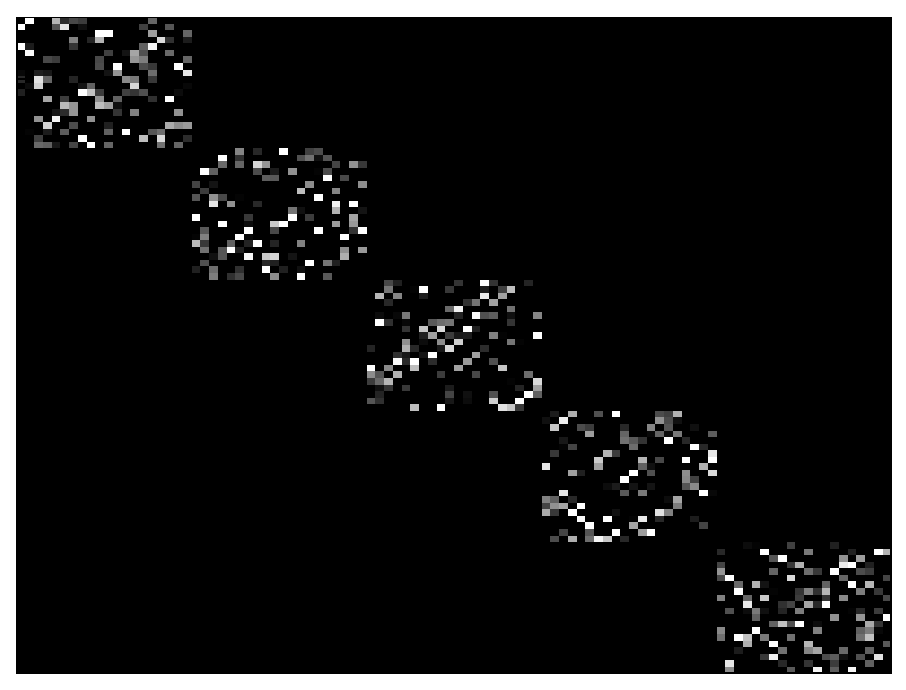
\includegraphics[width=\textwidth]{SEP}
    \caption{子空间自表示性满足}
  \end{subfigure}
  \begin{subfigure}[b]{0.4\textwidth}
    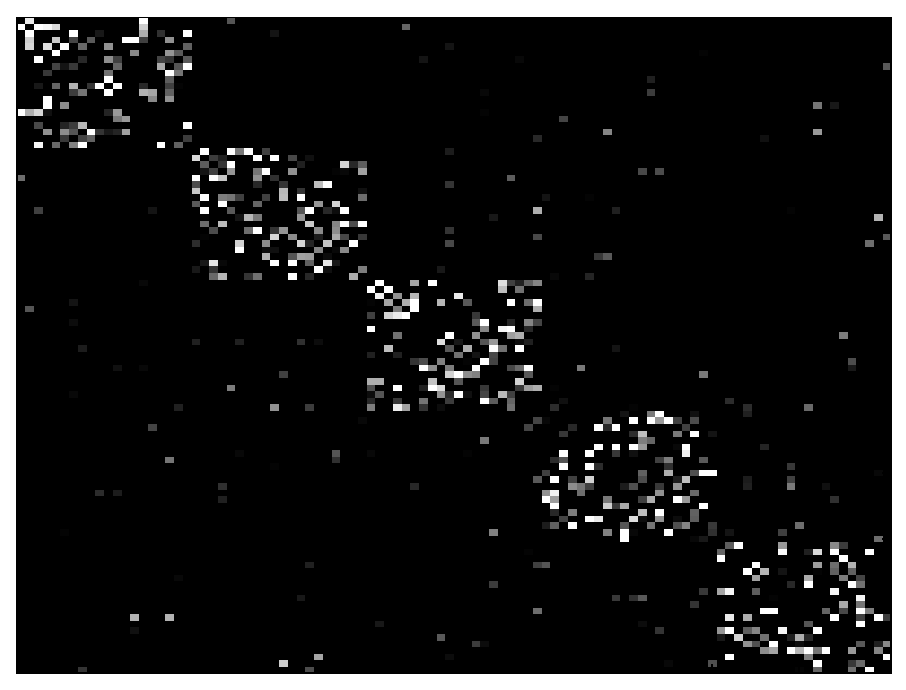
\includegraphics[width=\textwidth]{ViolateSEP}
    \caption{自表示性不满足}
  \end{subfigure}
  \caption{满足和不满足自表示性的邻接矩阵}
  \label{fig:SEP}
\end{figure}

\subsection{自表示的一般性条件}
我们不直接分析\eqref{eq:multi}, 而是引入松弛变量\(E\), 将其转化为有约束的等价形式:
\begin{equation}\label{eq:Opt_original}
  \mathbf{P}_0:\quad \min_{C, E} \;
  \|C^T\|_{2,1}+\frac{\lambda}{2}\|E\|_F^2 \quad
  \text{s.t.} \quad X_\cI=X_{\cI\rightarrow 0}C+E.
\end{equation}
\eqref{eq:Opt_original} 的对偶问题为:
\begin{equation}\label{eq:Opt_original_dual}
  \mathbf{D}_0:\quad \max_{N} \; \langle N, X_\cI\rangle -
  \frac{1}{2\lambda}\|N\|_F^2 \quad
  \text{s.t.} \quad \|N^T X_{\cI\rightarrow 0}\|_{2,\infty} \leq 1.
\end{equation}

先考虑一个一般的凸优化问题:
\begin{equation}\label{eq:Opt_A_general}
  \quad \min_{C, E} \; \|C^T\|_{2,1}+\frac{\lambda}{2}\|E\|^2_F \quad
  \text{s.t.} \quad B=AC+E.
\end{equation}
我们有\autoref{lemma:OptimalCondition},它是
\cite[引理~7.1]{soltanolkotabi2012geometric}的拓展.
\begin{lemma}\label{lemma:OptimalCondition}
  给定矩阵\(A\in \R^{d\times n}, B \in \R^{d\times m}\)和指标集\(\cT\subset [n]\),
  若存在矩阵 \(C\in \R^{n\times m},E\in \R^{d\times m}\) 使 \(B=AC+E\)成立, 且
  \(C\) 的行支撑集 \(\cJ\subseteq
  \cT\),同时又存在矩阵\(N\in\R^{d\times m}\)满足
  \begin{align*}
    N^T A_\cJ = \norm(C_{(\cJ)}^T),  & \quad N=\lambda E, \\
    \|N^T A_{\cT\cap \cJ^{c}}\|_{2, \infty} \leq 1, & \quad \|N^T A_{\cT^{c}}\|_{2, \infty}<1,
  \end{align*}
  其中 \(\norm(\cdot)\)是将矩阵的每一非零列归一化为单位向量,
  则\eqref{eq:Opt_A_general} 的最优解\((C^{*},E^{*})\) 必然有
  \(C^*_{(\cT^c)}=\mathbf{0}\).
\end{lemma}
\begin{proof}
  对最优解 \((C^{*},E^{*})\), 我们有:
  \begin{align}
    \|(C^*)^T\|_{2,1}+\frac{\lambda}{2}\|E^*\|_F^2 =& \|(C^*)^T_{(\cJ)}\|_{2,1}+\|(C^*)^T_{(\cT\cap \cJ^c)}\|_{2,1}+
    \|(C^*)^T_{(\cT^c)}\|_{2,1} + \frac{\lambda}{2} \|E^*\|^2_F\nonumber\\
    \geq&\|C^T_{(\cJ)}\|_{2,1}+\langle \norm(C^T_{(\cJ)}),(C^*)^T_{(\cJ)}-C^T_{(\cJ)}
    \rangle+\|(C^*)^T_{(\cT^c)}\|_{2,1}\nonumber \\
    &+\|(C^*)^T_{(\cT\cap \cJ^c)}\|_{2,1}+\frac{\lambda}{2} \|E\|^2_F +\langle
    \lambda E,E^*-E\rangle\nonumber\\
    =&\|C^T_{(\cJ)}\|_{2,1}+\langle N,A_\cJ(C^*_{(\cJ)}-C_{(\cJ)})\rangle
     +\|(C^*)^T_{(\cT\cap\cJ^c)}\|_{2,1}\nonumber\\
     &+\|(C^*)^T_{(\cT^c)}\|_{2,1} + \frac{\lambda}{2} \|E\|^2_F +\langle
    \lambda E,E^*-E\rangle\nonumber\\
    =&\|C^T_{(\cJ)}\|_{2,1}+\frac{\lambda}{2} \|E\|_F^2+ \|(C^*)^T_{(\cT\cap
    \cJ^c)}\|_{2,1}+\|(C^*)^T_{(\cT^c)}\|_{2,1}\nonumber\\
    &-\langle N,A_{T\cap \cJ^c}C^*_{(\cT\cap \cJ^c)}\rangle
    -\langle N,A_{\cT^c}C^*_{(\cT^c)}\rangle.
    \label{eq:lemma_tmp1}
  \end{align}
  其中 \(\frac{\lambda}{2} \|E^*\|_F^2 \geq \frac{\lambda}{2} \|E\|_F^2 +\langle
  \lambda E,E^*-E\rangle\) 可由Cauchy–Schwarz不等式推得.
  最后一个等式成立是因为 \((C,E)\)和\((C^*,E^*)\)都是可行解, 因此\(\langle
  N,A(C^*-C)\rangle+\langle N,E^*-E\rangle = \langle
  N,AC^*+E^*-(AC+E)\rangle=0\), 同时注意到 \(\| C^T_{(\cJ)}\|_{2, 1} = \|C^T\|_{2, 1}\).

  使用 \(N\) 的不等式条件, 我们有
  \begin{align*}
    \langle N,A_{\cT^c}C^*_{(\cT^c)}\rangle&= \langle A_{\cT^c}^TN,C^*_{(\cT^c)}\rangle
    \leq \|N^T
    A_{T^{c}}\|_{2,\infty}\|(C^*)^T_{(\cT^c)}\|_{2,1}, \\
    \langle N,A_{T\cap \cJ^c}C^*_{(\cT\cap \cJ^c)}\rangle&= 
    \langle A_{T\cap \cJ^c}^TN,C^*_{(\cT\cap \cJ^c)}\rangle
    \leq \|N^T A_{T\cap \cJ^{c}}\|_{2,\infty}\|(C^*)^T_{(\cT\cap
    \cJ^c)}\|_{2,1}. 
  \end{align*}
  将其带入 \eqref{eq:lemma_tmp1}, 我们得到:
  \begin{equation*}
    \|(C^*)^T\|_{2,1}+\frac{\lambda}{2} \|E^*\|^2_F \geq \|C^T\|_{2,1}+ \frac{\lambda}{2} 
    \|E\|_F^2 +(1-\|N^T A_{\cT^c}\|_{2, \infty})\|(C^*)^T_{(\cT^c)}\|_{2,1},
  \end{equation*}
  其中 \((1-\|N^T A_{\cT^c}\|_{2, \infty})\) 严格大于 \(0\).

  由于 \((C^*,E^*)\) 是最优解, \(\|(C^*)^T\|_{2,1}+\frac{\lambda}{2}
  \|E^*\|_F^2\leq \|C^T\|_{2, 1}+\frac{\lambda}{2} \|E\|_F^2\). 
  因此 \(\|(C^*)^T_{(\cT^c)}\|_{2,1}=0\) 且 \((C,E)\) 也是最优解.
\end{proof}

因为\(\Omega\)满足\eqref{eq:nosame}, 那么对\(\cI\in \Omega\),
存在\(\cS_\ell\) 满足\(y_i \in \cS_\ell, \, \forall i \in \cI\). 
若取\eqref{eq:Opt_A_general}中的\(B=X_\cI, A=X_{\cI\rightarrow 0}, \cT=\cI_\ell\),
则如果能构造三元组\((C,E,N)\), 满足\autoref{lemma:OptimalCondition} 的条件,
并且\(C_{(\cI_\ell^c)}=\mathbf{0}\). 那么\eqref{eq:Opt_original} 的最优解
\(C^*_{(\cI_\ell^c)}=\mathbf{0}\), 再保证\(C^*\)非平凡(不全为零)就可得到自表示性.

\subsection{构造三元组}\label{sec:construct_nu}
为了构造满足条件的三元组,我们希望将表示系数限制在同类点上,于是考虑下面\emph{假想}
\footnote{由于我们不知道每个点的类别,所以实际上无法求解这个问题,因此叫做``假想''}
的优化问题及其对偶问题:
\begin{align}\label{eq:Opt_fictitious2}
  \bP_1: \quad &\min_{C, E} \;
  \|C^T\|_{2,1}+\frac{\lambda}{2}\|E\|_F^2 \quad
  \text{s.t.} \quad X_\cI=X^{(\ell)}_{\cI^c}C+E,\\
  \bD_1: \quad &\max_{N} \; \langle X_\cI, N\rangle -
  \frac{1}{2\lambda} \|N\|_F^2 \quad
  \text{s.t.} \quad \|N^T X^{(\ell)}_{\cI^c}\|_{2, \infty} \leq 1.
  \label{eq:dual_fictitious2}
\end{align}
因为\(\left\{y_i : \forall i \in \cI \right\}\subset \cS_\ell\),
所以\(\bP_1\)相当于只用\(\cS_\ell\)中的数据来表示\(X_\cI\).

\eqref{eq:Opt_fictitious2}是有可行解的(我们只需要任取\(C_0\).
算出相应的\(E_0\), \((C_0, E_0)\)即为可行解), 因此由Slater条件\cite{boyd2004convex},
\eqref{eq:Opt_fictitious2}和\eqref{eq:dual_fictitious2}强对偶,
即\eqref{eq:Opt_fictitious2}的最优解\((C, E)\)与\eqref{eq:dual_fictitious2}最优解\(N\)满足
\begin{align}\label{eq:strong_dual}
  \|C^T\|_{2,1}+\frac{\lambda}{2}\|E\|_F^2 = \langle X_\cI,N \rangle -
  \frac{1}{2\lambda} \|N\|_F^2   
\end{align}
将\(X_\cI=X^{(\ell)}_{\cI^c}C+E\)代入\eqref{eq:strong_dual},稍加整理后得到
\[ \frac{1}{2}\| \sqrt{\lambda}E-\frac{1}{\sqrt{\lambda}}N \|_F^2+
\|C^T\|_{2,1}-\langle C^T, N^T X^{(\ell)}_{\cI^c}\rangle = 0. \]
设\(C\)的行支撑为\(\cJ\), 由\(\|N^T X^{(\ell)}_{\cI^c}\|_{2, \infty} \leq 1\),可得
\begin{align*}
  N=\lambda E, \quad (N^T X^{(\ell)}_{\cI^c})_\cJ =\norm(C_{(\cJ)}^T).
\end{align*}
\(C\in \R^{(n_\ell-m)\times m}\) 对应点\(\{ x_i: i \in \cI_\ell \setminus \cI\}\)
的表示系数, 所以我们将\(C\)按行扩充一些零向量得到\(C^*\)满足
\[ C^*_{\cI_\ell \setminus \cI} = C, \quad C^*_{(i)} = \mathbf{0}
\quad \forall i \in \cI^c_\ell \cup \cI. \]
则\((C^*, E)\)是\eqref{eq:Opt_original} 的可行解, 同时三元组\((C^*, E, N)\)
满足了\autoref{lemma:OptimalCondition} 的条件, 除了
\begin{equation*}
  \left\|N^T X_{\cI_\ell^c}\right\|_{2,\infty}<1,
\end{equation*}
即我们要给出条件使 \(\forall x \in \mathcal{X}\setminus \mathcal{X}^{(\ell)}\),有
\begin{equation}\label{eq:dual_separation_condition}
   \left \| N^T x\right \|_2 < 1.
\end{equation}
这样根据\autoref{lemma:OptimalCondition} 我们得到的可行解\((C^*, E)\)
就是\eqref{eq:Opt_original}的最优解, 再保证\(C^*\)非平凡, 则自表示性成立.

\subsection{对偶矩阵的限制}\label{sec:dual_separation}
我们将 \(N\) 的每一列在子空间 \(\mathcal{S}_{\ell}\) 上投影,得到 \(N_{\parallel}
:=\mathbb{P}_{\cS_\ell}N\), \(N_{\perp} := \P_{\cS_{\ell}^\perp}N\).因此
\begin{align}\label{eq:showing_dual_sep_cond}
  \| N^T x \|_2 =& \| N^T (y+z)\|_2 \leq \| N_{\parallel}^T y\|_2+\|
  N_{\perp}^T y\|_2+\|N^T z\|_2 \nonumber\\
  \leq& \mu(\mathcal{X}_{\ell}) \|N_{\parallel}\|_2 + \|N_{\perp}\|_2\|y\|_2
  + \|N_{\parallel}^T \P_{\cS_{\ell}} z\|_2 
  + \|N_\perp^T \P_{\cS_\ell^\perp} z\|_2 .
\end{align}
最后一个不等号是根据\autoref{def:incoherence}, 对\(N_\parallel\)做奇异值分解
\(N_\parallel = U\Sigma V^T\), 则
\[
  \|N_\parallel^T y\|_2 = \|V \Sigma U^T y\|_2 = \|\Sigma U^T y\|_2 \le
  \|N_\parallel\|_2 \left\|\P_{\cU_\cI^{(\ell)}} y\right\|_2 \le \mu(\cX_\ell)
  \|N_\parallel\|_2.
\]

\subsubsection{控制 \(\|N_{\parallel}\|_2\)}
我们考察\(N\) 在 \eqref{eq:dual_fictitious2}中的可行区域:
\[\left\{N \middle| \|N^T X^{(\ell)}_{\cI^c}\|_{2,\infty} \leq 1\right\},\]
等价于
\[\left\{N \middle| \| N^T x_i\|_2 \leq 1 \quad \forall \, i \in \cI_\ell
\setminus \cI \right\}.\]
分解可得
\[\| N_{\parallel}^T y_i+N_{\parallel}^T (\mathbb{P}_{\mathcal{S}_{\ell}}z_i)+
N_{\perp}^T z_i\|_2 \leq 1.\]
由三角不等式
\begin{equation}\label{eq:relax_constraint}
  \left\| N_{\parallel}^T y_i+N_{\parallel}^T
  (\mathbb{P}_{\mathcal{S}_{\ell}}z_i)\right \|_2
  \leq 1+\|N_{\perp}^T z_i\|_2 \leq 1+\delta\|N_{\perp}\|_2.
\end{equation}

根据多胞体的几何性质,我们有
\begin{align}
  & \| N_{\parallel}^T (y_i+ \mathbb{P}_{\mathcal{S}_{\ell}}z_i) \|_2 \leq
  1+\delta\|N_{\perp}\|_2 \quad \forall i \in \cI_\ell \setminus \cI\nonumber\\
  \Leftrightarrow & \|N_{\parallel}^T x\| \leq 1 \quad \forall x \in \mathcal{P}\left(\frac{Y_{\cI^c}^{(\ell)}+
  \P_{\mathcal{S}_{\ell}}(Z_{\cI^c}^{(\ell)})}{1+\delta\|N_{\perp}\|_2}\right)
  \nonumber\\
  \Rightarrow & \|N_{\parallel}^T x\| \leq 1 \quad \forall x \in \cS_\ell,
  \|x\|_1 \le r\left(\mathcal{P}\left(\frac{Y_{\cI^c}^{(\ell)}+
  \P_{\mathcal{S}_{\ell}}(Z_{\cI^c}^{(\ell)})}{1+\delta\|N_{\perp}\|_2}\right),
  \cS_\ell\right).\label{eq:Geometric_dual}
\end{align}
注意到\(\cP(\cdot)\) 是对称凸包, \(\cP(\cdot)\) 的最大内接球中心在原点.
由于这里都是对子空间\(\cS_\ell\)讨论, 简单起见, 记\(r(\cP, \cS)\)为\(r(\cP)\).
凸包的内接球半径大小能度量点在子空间中分布的均匀程度.
如\autoref{fig:inradius}所示, 不考虑噪音, 高维空间的三个点\(x_1, x_2,
x_3\)分布在一个二维平面的单位球面上, 当它们分布均匀时, 张出的对称凸包的半径较大, 反之
不均匀时, 半径较小. 内接球半径大说明, 在子空间的各个方向上数据点都有分布,
这样自然能更好地做稀疏表示.

\begin{figure}[tb]
  \centering
  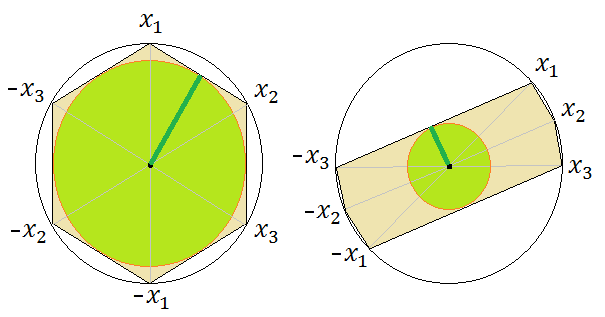
\includegraphics[width=0.8\linewidth]{inradius}
  \caption{数据点分布和其内接球半径的关系}
  \label{fig:inradius}
\end{figure}

我们可以通过子空间\(\cS_\ell\)中无噪音点\(Y^{(\ell)}_{\cI^c}\)的内接球半径控制\(\|N_{\parallel}\|_2\).
\begin{lemma}\label{lemma:circum_inradius}
  对于矩阵 \(A \in \R^{d \times n}\)和子空间\(\cS\subset \R^d\), 
  若\(A\)的每一列\(A_i \in \cS\) 且存在\(r>0\),使得
  \[\|A^Tx\|_2 \leq 1 \quad \forall x \in \cB(0, r)\cap \cS,\]
  其中\(\cB(0, r)\) 表示 \(\R^d\) 中的半径为\(\alpha\)的欧式球,
  那么\(\|A\|_2 \leq \frac{1}{\alpha}\).
\end{lemma}
\begin{proof}
  根据定义我们有
  \begin{align*}
    \|A\|_2 = \max_{x\in \R^n} \frac{\|A^Tx\|_2}{\|x\|_2}
    = \max_{x \in \cS} \frac{\|A^Tx\|_2}{\|x\|_2}
    = \max_{x \in \cB(0,r) \cap \cS} \frac{1}{r} \|A^Tx\|_2
    \leq \frac{1}{\alpha}.
  \end{align*}
\end{proof}

\begin{lemma}\label{lemma:Y_containing_set}
  矩阵 \(Y, Z\in \R^{d \times n}\), 子空间\(\cS \subset \R^d\),
  \(Y\)的每一列在子空间\(\cS\)中,令\(\rho:=\max_{i}\|\P_\cS Z_i\|\),
  那么我们有:
  \begin{equation*}
    r(\cP(Y+\P_\cS Z)) \geq r(\cP(Y)) - \rho
  \end{equation*}
\end{lemma}
\begin{proof}
  令\(X=Y+Z\), 则\(Y+\P_\cS Z=\P_\cS X\). 根据定义\(\cP(\P_\cS X)\) 的边界是集合 \(\mathcal{B}:=
  \left\{y|y=\mathbb{P}_\mathcal{S} X c; \|c\|_1=1\right\}\).
  内接球是凸包内的最大球,因此 \(r(\mathcal{P}(\mathbb{P}_\mathcal{S} X)) =
  \min_{y\in \mathcal{B}} \|y\|\). 对\(y \in \mathcal{B} \) 我们给出下界:
  \begin{align*}
    \|y\| \geq& \|Yc\|-\|\mathbb{P}_\mathcal{S}Z c\|\geq r(\mathcal{P}(Y)) - {\sum}_j{\|\mathbb{P}_\mathcal{S}z_j}\||c_j|
    \geq r(\mathcal{P}(Y)) - \rho\|c\|_1.
  \end{align*}
  因此得证.
\end{proof}

根据\eqref{eq:Geometric_dual}, \autoref{lemma:circum_inradius} 和\autoref{lemma:Y_containing_set},
我们可给出\(N_{\parallel}\)的上界:
\begin{align}
  \|N_{\parallel}\|_2 \leq& \frac{1+\delta\|N_{\perp}\|_2}
  {r(\mathcal{P}(Y_{\cI^c}^{(\ell)}+\mathbb{P}_{\mathcal{S}_{\ell}}(Z_{\cI^c}^{(\ell)}))}
  \nonumber \\
  \leq& \frac{1+\delta\|N_{\perp}\|_2}{r{\left( \cQ_{\cI^c}^{(\ell)}\right)}-\delta_1}.\label{eq:nu1_bound}
\end{align}
这个上界依赖于 \(\|N_{\perp}\|_2\), 接下来我们将对其进行分析.

\subsubsection{控制\(\|N_{\perp}\|_2\)}
由于 \(N\) 是 \(\mathbf{D}_1\) 的最优解,由对偶问题的性质,我们有
\[ N=\lambda E=\lambda(X_\cI-X^{(\ell)}_{\cI^c}C). \]
将 \(N\) 投影到 \(\cS^{\perp}_{\ell}\), 我们得到
\(N_{\perp}=\lambda \P_{\cS_{\ell}^{\perp}}(X_\cI-X^{(\ell)}_{\cI^c}C)
= \lambda \mathbb{P}_{\mathcal{S}_{\ell}^{\perp}}(Z_\cI-Z^{(\ell)}_{\cI^c}C)\).
于是对任意\(y\in \R^d, \|y\|_2=1\)
\begin{align}
  \|N_{\perp}^T y\|_2 & \leq\lambda \left(\|\mathbb{P}_{\mathcal{S}_{\ell}^{\perp}}Z_\cI\|_2
  +\|C^T (\mathbb{P}_{\mathcal{S}_{\ell}^{\perp}}Z^{(\ell)}_{\cI^c})^T y\|_2\right)\nonumber\\
  & \leq \lambda\left( \sqrt{m} \delta + \|C^T \ty\|_2\right) \nonumber\\
  & \leq \lambda\left( \sqrt{m} \delta + \sum_j |\ty_j|\|C_{(j)}\|_2\right) \nonumber\\
  & \leq \lambda\left( \sqrt{m} \delta + \|\ty\|_{\infty}\|C^T\|_{2,1}\right) \nonumber\\
  & \leq \lambda \delta(\Cgl+\sqrt{m}) \leq \lambda\delta\sqrt{m}(\Cgl+1).
  \label{eq:bounding_nu2_0}
\end{align}
其中\(\ty=(\mathbb{P}_{\mathcal{S}_{\ell}^{\perp}}Z^{(\ell)}_{\cI^c})^Ty\),
而\(\|\ty\|_\infty \leq \|z_i\|_2 \|y\|_2 \leq
\delta\). 由\eqref{eq:bounding_nu2_0}得
\begin{align}
  \|N_{\perp}\|_2 = \max_{\|y\|_2=1} \|N^T y\|_2 \le \lambda\delta\sqrt{m}(\Cgl+1).
  \label{eq:bounding_nu2}
\end{align}

下面我们给出 \(\Cgl\)的上界.
因为 \((C,E)\) 是 \eqref{eq:Opt_fictitious2} 的最优解,所以对任何可行解 \((\tC ,\tE)\)
都有 \(\Cgl+\frac{\lambda}{2}\|E\|^2_F \leq \tCgl+\frac{\lambda}{2}\|\tilde{E}\|_F^2\).
令 \(\tC\) 为下面无噪音优化问题的解
\begin{align}\label{eq:Opt_y only}
\min_{c} \; \Cgl \quad
\text{s.t.} \quad Y_\cI=Y^{(\ell)}_{\cI^c}C,
\end{align}
由强对偶性,
\[\tCgl = \max_{N}\left\{\langle N,Y_\cI\rangle | \|N^T
Y^{(\ell)}_{\cI^c}\|_{2, \infty}\leq 1\right\}.\]
根据\autoref{lemma:circum_inradius}, 对偶问题的最优解 \(\tilde{N}\) 满足
\(\|\tilde{N}\|_2 \leq \frac{1}{r(\mathcal{Q}_{\cI^c}^{(\ell)})}\).于是
\[\tCgl = \langle\tilde{N},Y_\cI\rangle \leq
\frac{m}{r(\mathcal{Q}_{\cI^c}^{(\ell)})}.\]

同时 \(\tilde{E} = Z_\cI - Z_{\cI^c}^{(\ell)}\tC\), 所以 
\[\|\tilde{E}\|_F^2 \leq (\|Z_\cI\|_F+\sum_{j,k} \|z_j\||\tC_{j,k}|)^2
\leq \delta^2 (\sqrt{m} + \|\tC\|_1)^2\leq m \delta^2(1+ \tCgl)^2,\]
于是
\begin{align}
  \Cgl \leq& \tCgl +
  \frac{\lambda}{2}\|\tilde{E}\|_F^2-\frac{\lambda}{2}\|E\|_F^2\nonumber \\
  \leq& \frac{m}{r{(\mathcal{Q}_{\cI^c}^{(\ell)})}}+\frac{\lambda}{2}m\delta^2
  \left[1+\frac{m}{r{(\mathcal{Q}_{\cI^c}^{(\ell)})}}\right]^2-\frac{1}{2\lambda}\|N_{\perp}\|_2^2,
  \label{eq:c_bound}
\end{align}
注意到 \(\frac{\lambda}{2}\|E\|_F^2=\frac{1}{2\lambda}\|N\|_F^2
\geq\frac{1}{2\lambda}\|N_{\perp}\|_F^2 \geq\frac{1}{2\lambda}\|N_{\perp}\|_2^2\).
将\eqref{eq:c_bound}带入 \eqref{eq:bounding_nu2}得
\[\|N_{\perp}\|_2 \leq \lambda \delta \sqrt{m} 
\left(\frac{m}{r(\mathcal{Q}_{\cI^c}^{(\ell)})}+\frac{\lambda}{2}\delta^2m
\left[1+\frac{m}{r(\mathcal{Q}_{\cI^c}^{(\ell)})}\right]^2+1\right)
-\frac{\delta}{2}\sqrt{m}\|N_{\perp}\|_2^2 \]
对上式稍加整理得到
\[\|N_{\perp}\|_2+\frac{\delta}{2}\sqrt{m}\|N_{\perp}\|_2^2\leq
  \lambda\delta\sqrt{m}\left(\frac{m}{r(\mathcal{Q}_{\cI^c}^{(\ell)})}+1\right)+
  \frac{\delta}{2}\sqrt{m} \left[\lambda\delta\sqrt{m}
  \left(\frac{m}{r(\mathcal{Q}_{\cI^c}^{(\ell)})}+1\right)\right]^2,\]
由于函数 \(f(\alpha)=\alpha+\frac{\delta}{2}\sqrt{m}\alpha^2\) 在 \(\alpha>0\)
时单调递增,则上面的不等式可以推出
\begin{equation}\label{eq:nu2_bound}
  \|N_{\perp}\|_2 \leq \lambda\delta\sqrt{m}\left(\frac{m}{r(\mathcal{Q}_{\cI^c}^{(\ell)})}+1\right),
\end{equation}
即我们需要的 \(\|N_{\perp}\|_2\) 的上界.

\subsubsection{ \(\|N^T x\|_2<1\) 所需的条件}
结合 \eqref{eq:showing_dual_sep_cond}, \eqref{eq:nu1_bound} 和 \eqref{eq:nu2_bound}, 
我们可以得出 \(\|N^T x\|_2\) 的上界:
\begin{align*}
  \|N^T x\|_2 \leq& (\mu(\mathcal{X}_{\ell})+\|\mathbb{P}_{\mathcal{S}_{\ell}}z\|) 
  \|N_{\parallel}\|_2+(\|y\|+\|\mathbb{P}_{\mathcal{S}_{\ell}^{\perp}}z\|)\|N_{\perp}\|_2\\
  \leq&\frac{\mu(\cX_\ell)+\delta_1}{r{\left(\cQ_{\cI^c}^{(\ell)}\right)}-\delta_1}
  +\left(\frac{(\mu(\mathcal{X}_{\ell})+\delta_1)\delta}{r{\left( \mathcal{Q}_{\cI^c}^{(\ell)}\right)}-\delta_1}+1+\delta\right)
  \|N_{\perp}\|_2\\
  \leq& \frac{\mu(\mathcal{X}_{\ell})+\delta_1}{r{\left( \mathcal{Q}_{\cI^c}^{(\ell)}\right)}-\delta_1} +
  \lambda\delta(1+\delta)\sqrt{m}
  \left(\frac{m}{r(\mathcal{Q}_{\cI^c}^{(\ell)})}+1\right) \\
  &+ \frac{\lambda\delta^2\sqrt{m}(\mu(\mathcal{X}_{\ell})+\delta_1)}
  {r{\left( \mathcal{Q}_{\cI^c}^{(\ell)}\right)}-\delta_1}\left(\frac{m}{r(\mathcal{Q}_{\cI^c}^{(\ell)})}+1\right).
\end{align*}
简单起见,我们把第二个 \(r(\mathcal{Q}_{\cI^c}^{(\ell)})\) 松弛成 \(r(\mathcal{Q}_{\cI^c}^{(\ell)})-\delta_1\).
这样对偶分离条件就被下式保证
\begin{multline}\label{eq:dual_cond_full}
   \lambda\sqrt{m}\delta(1+\delta)
  +\frac{\lambda\delta^2 m^{3/2}(\mu(\mathcal{X}_{\ell})+\delta_1)}
  {r{\left( \mathcal{Q}_{\cI^c}^{(\ell)}\right)}(r{\left(
    \mathcal{Q}_{\cI^c}^{(\ell)}\right)}-\delta_1)} \\
  +\frac{\mu(\mathcal{X}_{\ell})+\delta_1 +\lambda m^{3/2}\delta(1+\delta)+
  \lambda\sqrt{m}\delta^2(\mu(\mathcal{X}_{\ell})+\delta_1)}
  {r{\left( \mathcal{Q}_{\cI^c}^{(\ell)}\right)}-\delta_1}<1.
\end{multline}
记 \(\rho:=\lambda\sqrt{m}\delta\), 假设\(\delta<r{\left(\cQ_{\cI^c}^{(\ell)}\right)}\)
和\((\mu(\mathcal{X}_{\ell})+\delta_1)<1\), 那么我们有下面的不等式
\begin{align*}
  \frac{\lambda\sqrt{m}\delta^2(\mu(\mathcal{X}_{\ell})+\delta_1)}
  {r{\left( \mathcal{Q}_{\cI^c}^{(\ell)}\right)}-\delta_1}
  +\frac{\lambda\delta^2 m^{3/2}(\mu(\mathcal{X}_{\ell})+\delta_1)}
  {r{\left( \mathcal{Q}_{\cI^c}^{(\ell)}\right)}(r{\left( \mathcal{Q}_{\cI^c}^{(\ell)}\right)}-\delta_1)}
  < \frac{\rho (m+\delta)}{r{\left( \mathcal{Q}_{\cI^c}^{(\ell)}\right)}-\delta_1}.
\end{align*}
用上式化简\eqref{eq:dual_cond_full} 左边, 可得一个充分条件
\begin{equation}\label{eq:dual_cond_simp}
  \mu(\mathcal{X}_{\ell}) +\rho [2m+(1+m)\delta] +\delta_1
  < \left(1-\rho(1+\delta)\right)(r(\mathcal{Q}_{\cI^c}^{(\ell)})-\delta_1).
\end{equation}
把 \eqref{eq:dual_cond_simp} 一般化到所有子空间的所有分组上,
则必须对每个\(\ell = 1,...,L\) 成立:
\begin{equation}\label{eq:Thm1_all}
  \mu(\mathcal{X}_{\ell}) +\rho [2m+(1+m)\delta] +\delta_1
  < \left(1-\rho(1+\delta)\right)\left(\min_{\{\cI: \cI\in \Omega_\ell\}}r(\mathcal{Q}^{(\ell)}_{\cI^c})-\delta_1\right).
\end{equation}

\subsection{避免平凡解}\label{sec:avoid_trivial}
除了满足自表示以外, 我们还要要求解是非平凡的. 不难看出,只要当 \(\lambda\)
足够大时, 平凡解 \((\mathbf{0}, X_\cI)\) 肯定不是最优解.

\begin{lemma}\label{lemma:avoid_trivial}
  对于 \eqref{eq:Opt_A_general} ,当 \(\lambda > \frac{1}{\max_{i,j} |A_i^T
B_j|}\) 时,其最优解一定是非平凡的.
\end{lemma}
\begin{proof}
  我们只要说明存在一个非平凡解比平凡解更优即可. 设 \(i, j\) 为 \(|A_i^T
  B_j|\) 取到最大时的下标, 构造可行解\(C\), 
  取\(C_{i,j} = \frac{\lambda |A_i^T B_j|-1}{\lambda \|A_i\|_2^2} \sign(A_i^T B_j)\) 
  其余为\(0\), 则\(C\) 非平凡.我们有
  \begin{align*}
    \frac{\lambda}{2} \|B_j - A_i C_{i, j} \|_2^2 + |C_{i, j}| =& \frac{\lambda}{2}
    \|B_j\|_2^2 + \frac{\lambda}{2} \|A_i\|_2^2 C_{i,j}^2 +\left( 1-\lambda |A_i^T B_j|
    \right)C_{i,j} \\
    =&\frac{\lambda}{2} \|B_j\|_2^2 - \frac{(\lambda|A_i^T B_j| -1)^2}
    {2 \lambda \|A_i\|_2^2 }\\
    <& \frac{\lambda}{2} \|B_j\|_2^2. 
  \end{align*}
  因此最优解一定非平凡.
\end{proof}

我们要求\eqref{eq:Opt_fictitious2} 的解非平凡, 因此需要考虑
\(\|[X_{\cI^c}^{(\ell)}]^T X_\cI \|_{\infty} \).
设\(i, i_0\in \cI_\ell \setminus \cI, \, j, j_0\in
\cI\), 且
\begin{gather*}
x_{i_0}^T x_{j_0}=\left\|\left[X_{\cI^c}^{(\ell)}\right]^T X_\cI\right\|_\infty, \\
y_i^T y_j=\left\|\left[ Y_{\cI^c}^{(\ell)}\right]^T Y_\cI\right\|_\infty ,
\end{gather*}
则
\begin{align}
  \left\|[X_{\cI^c}^{(\ell)}]^TX_\cI\right\|_{\infty}&=\left|\langle x_{i_0},
  x_{j_0}\rangle\right|  \geq \left|\langle x_i, x_j\rangle\right|\nonumber\\
  &= \left|\langle y_i, y_j\rangle  + \langle y_i, z_j\rangle + \langle z_i, y_j\rangle + \langle z_i, z_j\rangle\right|\nonumber\\
  &\geq \left|\langle y_i, y_j\rangle\right| - \left|\langle y_i, z_j\rangle + \langle z_i, y_j\rangle + \langle z_i, z_j\rangle\right|\nonumber\\
  & = \left\|[y_{\cI^c}^{(\ell)}]^Ty_i\right\|_{\infty} - \left|\langle y_i, z_j\rangle + \langle z_i, y_j\rangle + \langle z_i, z_j\rangle\right|\nonumber\\
  &\geq r(\mathcal{Q}^{(\ell)}_{\cI^c}) - 2\delta - \delta^2. \label{eq:lowerbounding_maX_affinity}
\end{align}
最后一个不等式成立是因为 \(\mathcal{Q}^{(\ell)}_{\cI^c}\) 
的内接球半径是集合 \(\{\| [ Y_{\cI^c}^{(\ell)}]^T w\|_\infty: w
\in  \mathcal{S}_{\ell}\} \) 的下界. 因此只要
\begin{equation}\label{eq:lambda_low}
  \lambda > \frac{1}{ r(\mathcal{Q}^{(\ell)}_{\cI^c}) - 2\delta - \delta^2},
\end{equation}
\eqref{eq:Opt_fictitious2}的解就是非平凡的.

\subsection{自表示定理}
将上面几小节的内容总结一下可以得到MT-SSC的自表示定理
\begin{theorem}\label{thm:mt_SEP}
  在带噪音的确定性模型下,若给定指标集\(\Omega\), 满足\eqref{eq:nointer}
  \eqref{eq:full} 和 \eqref{eq:nosame},且\(|\cI|=m, \, \forall\, \cI \in \Omega\).
  对任意\(\ell \in [L]\), 若\(\mu(\cX_\ell)<1-\delta_1\), \(\min_{\cI\in
  \Omega_\ell} r\left(\cQ^\ell_{\cI^c}\right) > \delta\), 同时能取出
  参数\(\lambda > \frac{1}{ r(\mathcal{Q}^{(\ell)}_{\cI^c}) - 2\delta -\delta^2}\),
  使得
  \[\mu(\cX_\ell) +\sqrt{m}\delta\lambda \left[2m+(1+m)\delta \right] +\delta_1
  < \left(1-\sqrt{m}\delta\lambda(1+\delta)\right)\left(\min_{\cI\in \Omega_\ell}
  r(\cQ^{(\ell)}_{\cI^c})-\delta_1\right)\]
  成立. 那么MT-SSC算法得到的解具有自表示性.
\end{theorem}
需要指出的是虽然在\autoref{thm:mt_SEP} 中\(m\)越大条件越不容易满足,
但是这并不代表MT-SSC表现一定比SSC差. 只是MT-SSC相对SSC不等式放缩更难处理,
所以得到的理论条件较苛刻.

\section{G-SSC的理论分析}\label{sec:proof_group}
类似于MT-SSC,我们希望能得到G-SSC算法结果
自表示的充分条件,简单起见,本节不考虑噪音.

将 \eqref{eq:group} 的限制条件去掉, 得到等价的优化问题
\begin{equation} \label{eq:group_nost}
  \min_{c} \|c\|_{\Omega,1}+\frac{\lambda}{2} \|x_i-X_{\{i\}\rightarrow
0}c\|_2^2,
\end{equation}
由于不考虑噪音, \eqref{eq:group_nost} 可以进一步简化为
\begin{equation} \label{eq:group_nonoise}
    \min_{c} \|c\|_{\Omega,1} \quad\text{s.t.}\quad
    Y_{\{i\}\rightarrow 0} c=y_i
\end{equation}
我们使用$Y$和$y_i$表示无噪音的数据点.

为了得到 \eqref{eq:group_nonoise} 的自表示条件,先考虑一般的优化问题
\[
  \bP_2(b,A): \,\, \min_c\, \| c\|_{\Omega,1} \quad \text{s.t.}\quad Ac = b
\]
其对偶问题为 
\[
  \bD_2(b,A): \,\, \max_{v}\, b^T v \quad
  \text{s.t.}\quad \|A^Tv\|_{\Omega,\infty} \leq 1
\]
其中某个向量$x$ 的$\|\cdot\|_{\Omega, \infty}$的范数定义为
$\max_{\cI \in \Omega} \|x_\cI\|_2$.

类似于MT-SSC, 我们先对一般的优化问题 $\bP_2(b,A)$ 进行分析.
\begin{lemma}\label{lem:prim_dual}
  给定矩阵$A\in\R^{d\times n}$, 向量$b\in \R^d$, 指标集$\cT\subseteq [n]$以及
  指标集族$\Omega$满足 \eqref{eq:nointer} 和 \eqref{eq:full},  
  且$\cT$是$\Omega$中某些指标集的并.
  若存在$c\in \R^n $使得$b = Ac$成立, $c$的支撑集$\cJ \subseteq \cT$,
  同时又存在$v\in\R^d$, 对$\forall \cI \in \Omega$有
  \begin{align}
    A^T_\cI v= \frac{c_\cI}{\|c_\cI\|_2} \quad& \text{if}\quad \cI \cap \cJ \neq
    \emptyset,\label{eq:group_c1}\\
    \|A^T_\cI v\|_2 \le  1 \quad &\text{if}\quad \cI \subseteq \cT,\label{eq:group_c2} \\
    \|A^T_\cI v\|_2< 1\quad &\text{if}\quad \cI \nsubseteq \cT\label{eq:group_c3}.
  \end{align}
  那么$\mathbf{P}_2(b,A)$的最优解$c^*$的支撑集$\cJ^*\subseteq \cT$.
\end{lemma}
\begin{proof}
  首先由于$\Omega$中的指标集两两交为空, 而$\cT$是$\Omega$中某些指标集的并, 
  所以对某个$\Omega$中的指标集$\cI$, 若$\cI \nsubseteq \cT$, 则
  $\cI \cap \cJ\subseteq \cI \cap \cT =\emptyset $, 因此 \eqref{eq:group_c1} 和 \eqref{eq:group_c3} 
  的不会矛盾.

  对于最优解$c^*$, 我们有
  \begin{align}
    \|c^*\|_{\Omega, 1} =& \sum_{\cI \cap \cJ\neq \emptyset}\|c^*_\cI\|_2 +
    \sum_{\cI \cap \cJ = \emptyset} \|c^*_\cI\|_2 \nonumber \\
    \ge& \sum_{\cI \cap \cJ\neq \emptyset}\|c_\cI\|_2 + 
    \sum_{\cI \cap \cJ\neq \emptyset}\langle \frac{c_\cI}{\|c_\cI\|_2} , c^*_\cI-c_\cI\rangle +
    \sum_{\cI \cap \cJ=\emptyset}\|c^*_\cI\|_2 \nonumber \\
    =& \sum_{\cI \cap \cJ\neq \emptyset}\|c_\cI\|_2 + 
    \sum_{\cI \cap \cJ\neq \emptyset}\langle v, A_\cI(c^*_\cI-c_\cI)\rangle +
    \sum_{\cI \cap \cJ =\emptyset}\|c^*_\cI\|_2 \nonumber \\
    =& \sum_{\cI \cap \cJ\neq \emptyset}\|c_\cI\|_2 +
    \sum_{\cI \cap \cJ = \emptyset} \left(\|c^*_\cI\|_2 -
    \langle v, A_\cI c^*_\cI\rangle\right),\label{eq:group_low1}
  \end{align}
  其中第一个不等号是因为$\|c^*_\cI\|_2 \ge \langle c_\cI/\|c_\cI\|_2,c^*_\cI\rangle$,
  第一个等号直接带入 \eqref{eq:group_c1} 可得,
  第二个等号是因为$c,c^*$满足$Ac=Ac^*=b$, 于是$\sum_{\cI\cap\cJ \neq
  \emptyset}A_\cI(c_\cI^*-c_\cI)=
  -\sum_{\cI \cap\cJ =\emptyset} A_\cI(c_\cI^*-c_\cI)$,
  而$c_{\cJ^c}=\mathbf{0}$, 所以带入可得. 由于
  $$\langle v, A_\cI c_\cI^*\rangle = \langle A_\cI^T v,
  c_\cI^*\rangle \le \|A_\cI^T v\|_2 \|c_\cI^*\|_2,$$
  所以 \eqref{eq:group_low1} 可以进一步放缩成
  \begin{align}
    \|c^*\|_{\Omega, 1} \ge& \sum_{\cI \cap \cJ\neq \emptyset}\|c_\cI\|_2 +
    \sum_{\cI \cap \cJ = \emptyset} \left(1-\|A_\cI^T v\|_2\right)\|c^*_\cI\|_2 \nonumber \\
    \ge& \|c\|_{\Omega, 1} + \sum_{\cI \nsubseteq \cT}\left(1-\|A_\cI^T
    v\|_2\right)\|c^*_\cI\|_2,
    \label{eq:group_low2}
  \end{align}
  其中用了 \eqref{eq:group_c2}.   因为$c^*$是最优解,
  所以$\|c^*\|_{\Omega,1}\le \|c\|_{\Omega, 1}$,
  结合 \eqref{eq:group_c3} 可得$c^*_\cI = \mathbf{0},\, \cI \nsubseteq \cT$.
\end{proof}

\subsection{自表示条件}
设点$y_i\in\cS_\ell$, 为了构造满足满足\autoref{lem:prim_dual} 条件的$c$和$v$,
我们先将优化问题的数据限制在子空间$\cS_\ell$中,
即先考虑$\bP_2(y_i, Y_{\cI_\ell^c\cup \{i\}\rightarrow 0})$.
$\bP_2(y_i, Y_{\cI_\ell^c\cup \{i\}\rightarrow 0})$
的最优解$c$满足$y_i=Y_{\{i\}\rightarrow 0}c$, 且支撑集$\cJ \subseteq \cI_\ell$,
而由强对偶性可得$\bD_2(y_i, Y_{\cI_\ell^c\cup \{i\}\rightarrow 0})$的最优解$v$,
对$ \cI\in \Omega$ 满足
\begin{align*}
  (Y_{\{i\}\rightarrow 0})^T_\cI v = \frac{c_\cI}{\|c_\cI\|_2}, \quad&
  \text{if}\quad\cI \cap \cJ \neq \emptyset \\
  \|(Y_{\{i\}\rightarrow 0})^T_\cI v\|_2 \le 1, \quad&
  \text{if} \quad \cI \subseteq \cI_\ell 
\end{align*}
因此如果
\begin{equation} \label{eq:group_cond1}
  \|Y_\cI^T v\|_2<1, \quad \text{if} \quad\cI \nsubseteq \cI_\ell
\end{equation}
成立, 那么根据\autoref{lem:prim_dual},  $\bP_2(y_i, Y_{\{i\}\rightarrow 0})$
的最优解$c^*$有$c^*_{\cI_\ell^c}=\mathbf{0}$, 即满足自表示性.

我们把 \eqref{eq:group_cond1} 写成等价形式
\begin{equation*}
  \left\|Y_\cI^T \frac{v}{\|v\|_2}\right\|_2 \|v\|_2<1,
\end{equation*}
\(\|Y_\cI v/\|v\|_2\|_2\)由子空间之间的不相干性控制, 所以我们主要考察
$\|v\|_2$的上界.由于$v$是$\bD_2(y_i, Y_{\cI_\ell^c\cup \{i\}\rightarrow 0})$
的最优解,而$Y_{\cI_\ell^c\cup \{i\}\rightarrow 0}$的非零列和$y_i$都在子空间
$\cS_\ell$中, 所以$\bD_2(y_i, Y_{\cI_\ell^c\cup \{i\}\rightarrow 0})$ 一定存在
最优解属于$\cS_\ell$. 不妨设$v\in \cS_\ell$, 同时$v$属于集合
$$\{ v: \|Y^T_{\cI_\ell^c\cup \{i\}\rightarrow 0} v\|_{\Omega,\infty}\le
1\}.$$
为了给出$\|v\|_2$的上界, 我们需要\autoref{lem:group_rR}. 
\begin{lemma}\label{lem:group_rR}
  给定矩阵$A\in \R^{d\times n}$, 指标集族$\Omega$和子空间$\cS\subset \R^d$,
  满足$A$中的每列$A_i\in \cS$, 定义集合
  \begin{align*}
    \cK &:= \left\{ Ab: \|b\|_{\Omega, 1}\le 1, b\in \R^n \right\},\\
    \cK^\circ &:= \left\{ u\in \cS : \|A^Tu\|_{\Omega, \infty}\le 1 \right\},
  \end{align*}
  则对 $u\in \cK^\circ$ 有
  $$ \|u\|_2 \le \frac{1}{r(\cK, \cS)}.$$
\end{lemma}
\begin{proof}
  $\cK$和$\cK^\circ$都是关于原点中心对称的凸包, 所以
  对任意$a\in \cS, \|a\|_2\le r(\cK, \cS)$, 有 $a \in \cK$,
  即存在$ b\in\R^n, \|b\|_{\Omega, 1}\le 1$, 使得$a=Ab$. 则$\forall u\in
  \cK^\circ$,
  有
  \begin{equation*}
    |a^T u| = |b^T A^T u| \le \sum_{\cI\in \Omega} \|b_\cI\|_2 \|A^T_\cI u\|_2
    \le \|b\|_{\Omega, 1}\|A^T u\|_{\Omega,\infty} \le 1.
  \end{equation*}
  由$a$的任意性可得
  $$ \|u\|_2 \le \frac{1}{r(\cK, \cS)}.$$
\end{proof}
根据\autoref{lem:group_rR}, 我们定义
\begin{equation*}
  \cQ_\Omega := \left\{ Y^T_{\cI_\ell^c\cup \{i\}\rightarrow 0}b:
  \|b\|_{\Omega, 1}\le 1, b\in \R^n \right\},
\end{equation*}
则 $\|v\|_2 \le 1/r(\cQ_\Omega, \cS_\ell)$.
因此, \eqref{eq:group_nonoise} 的解满足自表示性的充分条件为
\begin{equation} \label{eq:group_cond2}
  \left\|Y_\cI^T \frac{v}{\|v\|_2}\right\|_2 < r(\cQ_\Omega, \cS_\ell), \quad
  \cI \nsubseteq \cI_\ell, \forall\, \cI \in \Omega.
\end{equation}
如果我们把 \eqref{eq:group_cond2} 和\cite[定理~2.5]{soltanolkotabi2012geometric}
的条件$|\langle y_i, v/\|v\|_2\rangle|<r(\cQ^\ell_{-i}, \cS_\ell)$
相比较可以发现, \eqref{eq:group_cond2} 的不等式左右两项都较大, 所以理论上很难
判断那种算法更好.

\chapter{数值实验}\label{chp:experiments}
本章我们将提出的新方法运用到Hopkins155~\cite{tron2007benchmark} 和 NUS-WIDE
~\cite{chua2009nus} 数据集上, 并和SSC、LRR 比较, 说明新算法的优势.

\section{运动分割}
\begin{figure}[hb]
  \centering
  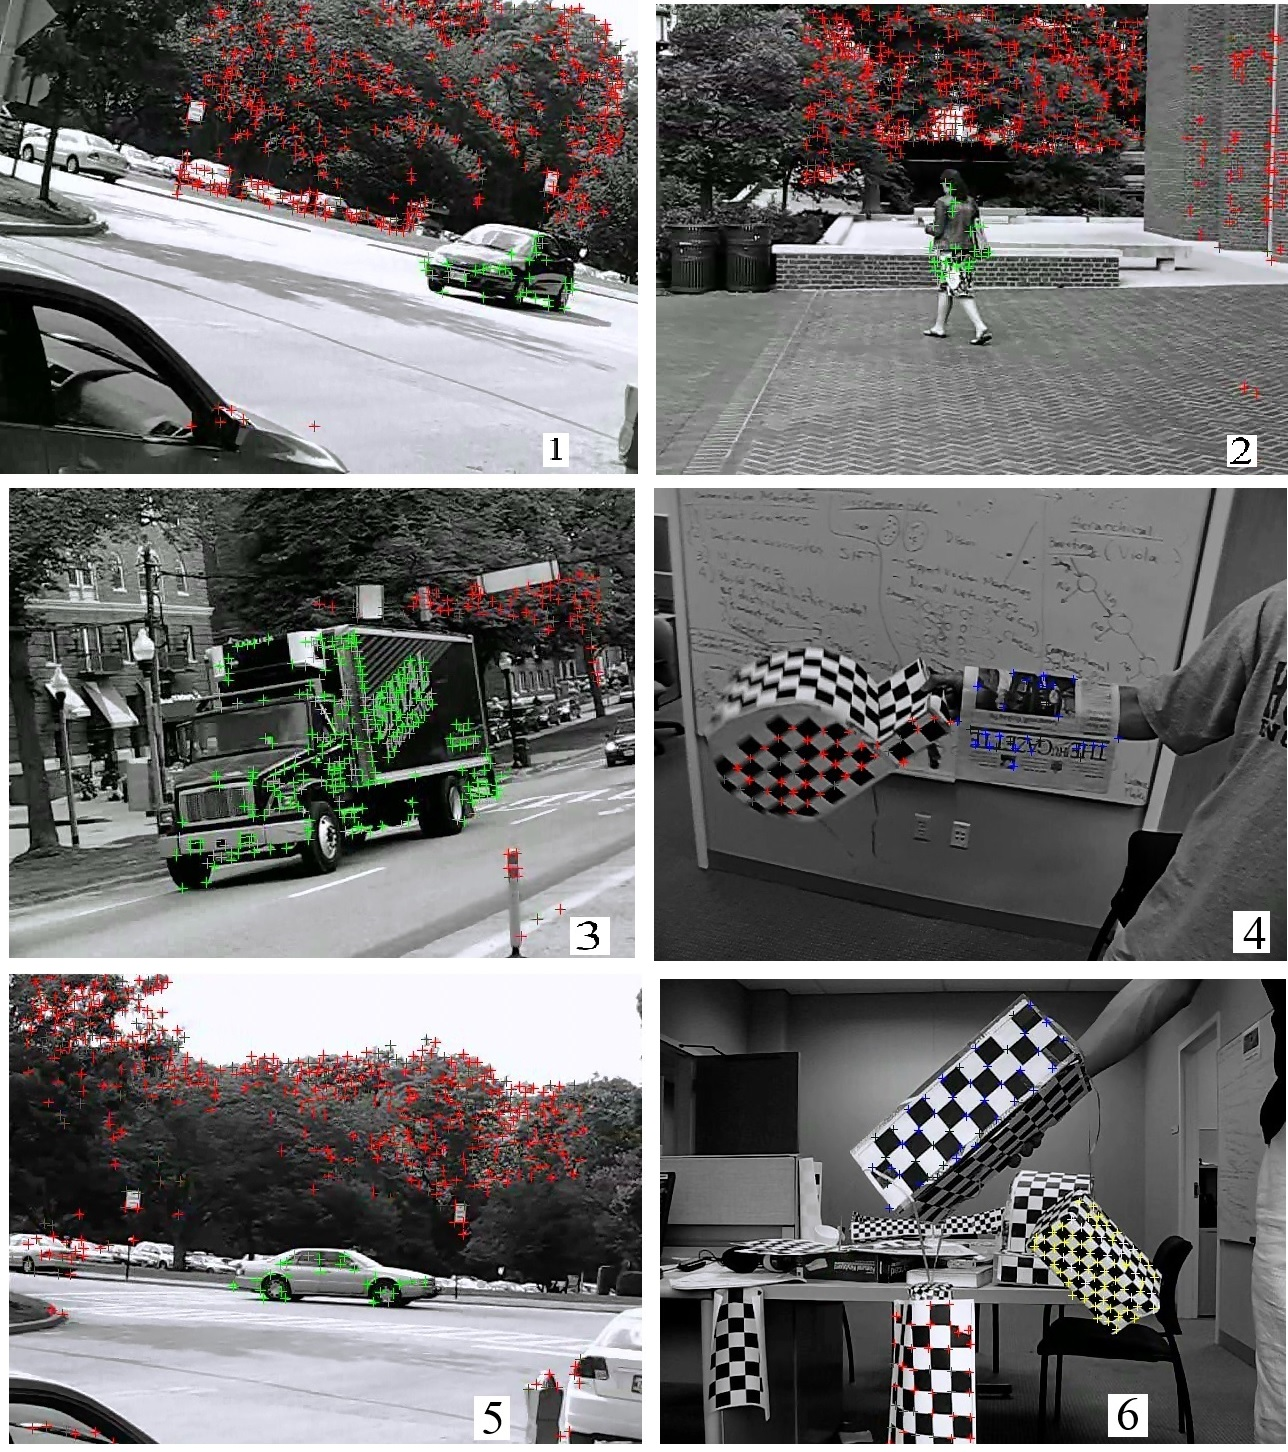
\includegraphics[width=0.7\textwidth]{hopkins}
  \caption{Hopkins155 中的视频某些帧}
  \label{fig:hopkins}
\end{figure}
Hopkins155数据集包含155个视频, 每个视频中有2或3个物体.
主要分成三种类型: 棋盘类, 如\autoref{fig:hopkins} 中4, 6所示,
人们手持棋盘状物体做各种运动, 用相机拍摄视频, 然后将棋盘点在每一帧中
的位置记录下来, 组成高维数据; 交通类, 如\autoref{fig:hopkins} 中1, 3, 5所示,
视频记录了两或三辆车的运动; 其他非刚性运动, 如\autoref{fig:hopkins} 中2所示,
包括人走路, 关节, 头部运动等.

从拍摄图中可以看出, 被跟踪的点来自多个运动实体, 如果把视频看作很多张顺序
图片, 那么每个被跟踪点都有一系列在图片中的相对位置. 我们要根据这些位置,
将每个点分类, 即将来自同一个运动实体的点归为一类.
\begin{table}[!htb]
  \centering
  \begin{tabular}{|c|c|c|c|c|}
	\hline
	算法 & SSC  & LRR  & MT-SSC        & G-SSC         \\ \hline \hline 
	棋盘(78组) &      &      &               &               \\
	平均数     & 2.12 & 2.79 & \textbf{1.83} & 1.91 \\
    中位数     & \textbf{0.51} & 0.72 & 0.57   &\textbf{0.51}  \\ \hline
	交通(31组) &      &      &               &               \\
	平均数     & 0.29 & 0.95 & \textbf{0.15} & 0.35          \\
    中位数     & \textbf{0.00} & \textbf{0.00} & \textbf{0.00}& \textbf{0.00} \\ \hline
	其他(11组) &      &      &               &               \\
    平均数     & \textbf{0.72} & 2.74 & 1.40          & 1.06          \\
    中位数     & \textbf{0.11} & 0.84 &\textbf{0.11} & \textbf{0.11}   \\ \hline
	所有2类数据  &      &      &               &               \\
	平均数     & 1.52 & 2.31 & \textbf{1.36} & 1.43 \\
    中位数     & \textbf{0.12} & 0.84 & \textbf{0.12} & \textbf{0.12}  \\ \hline
  \end{tabular}
  \caption{包含2个物体的数据聚类错误率(越低越好,单位\%)}
  \label{tab:hopkins2}
  \bigskip
  \begin{tabular}{|c|c|c|c|c|}
	\hline
	算法 & SSC  & LRR  & MT-SSC        & G-SSC         \\ \hline \hline
	棋盘(26组) &      &      &               &               \\
	平均数     & 2.97 & 4.47 & \textbf{2.09} & 2.37 \\
    中位数     & \textbf{0.30} & 0.50 & 0.34 & 0.34          \\ \hline
	交通(7组)  &      &      &               &               \\
    平均数     & \textbf{0.58} & 1.05 & 1.51          & 1.51          \\
    中位数     & \textbf{0.00} & 0.02 & \textbf{0.00}& \textbf{0.00}  \\ \hline
	其他(2组)  &      &      &               &               \\
	平均数     & 1.42 & 5.78 & \textbf{0.78} & 1.79          \\
	中位数     & 0.15 & 0.25 & \textbf{0.12} & \textbf{0.12} \\ \hline
	所有3类数据  &      &      &               &               \\
	平均数     & 2.45 & 3.71 & \textbf{1.82} & 2.10 \\
    中位数     & 0.24 & 0.40 & \textbf{0.14}  & 0.16  \\ \hline
  \end{tabular}
  \caption{包含3个物体的数据聚类错误率(越低越好,单位\%)}
  \label{tab:hopkins3}
\end{table}

\begin{figure}[tb]
  \centering
  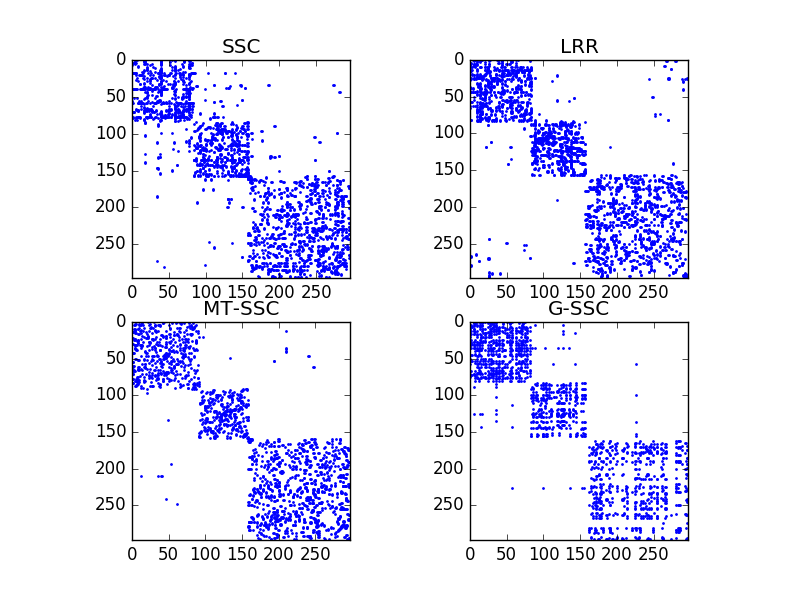
\includegraphics[width=\textwidth]{hopkins_W}
  \caption{SSC, LRR, MT-SSC和G-SSC在cars 10数据上的邻接矩阵}
  \label{fig:hopkins_neig}
\end{figure}
我们比较SSC\footnote{SSC的代码下载自http://vision.jhu.edu/code/.},
LRR\footnote{LRR 的代码下载自https://sites.google.com/site/guangcanliu/.},
MT-SSC,G-SSC四种算法在运动分割上的效果.
由于原始数据点集中在一个相对低维空间中, 导致分组算法很不稳定.
我们用PCA将数据降到\(4L\)维空间 (\(L\)是子空间类数), 并且将之白化(Whitening),
使每个特征有相同的方差. 
取\autoref{alg:nsn} 的参数\(r=2, k=5, \theta=0.05\),
这样得到的分组结果错误率(包含不同类点的分组数/总分组数)为\(0.0063\),
平均每组包含\(4.27\)个点.
进而对原始数据用MT-SSC和G-SSC聚类,
得到聚类错误率(将聚类结果与真实类别比较, 不匹配的点数/总点数)
见\autoref{tab:hopkins2} 和\autoref{tab:hopkins3}. 
可以看出在棋盘类数据中MT-SSC和G-SSC比SSC、LRR表现更优, 也因此总体结果更好.
我们选取一组数据画出了四种算法的邻接矩阵,如\autoref{fig:hopkins_neig} 所示,
相比于SSC,MT-SSC和G-SSC的错误连接更少, 说明其抗干扰能力更强.

\section{图片聚类}
\begin{figure}[htb]
  \centering
  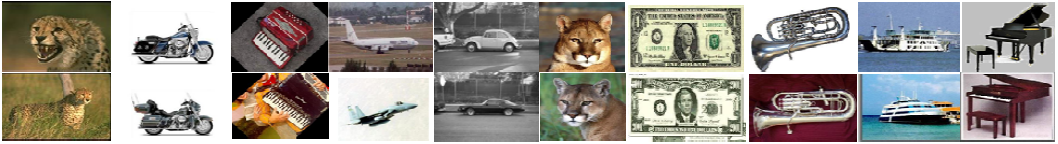
\includegraphics[width=\textwidth]{nusobj}
  \caption{10种物体的图片,这里每样展示了两张}
  \label{fig:nus}
\end{figure}
NUS-WIDE~\cite{chua2009nus} 数据集提供了269648张真实物体
和场景的照片,包括飞机、动物、建筑等等.
我们挑选了其中1000张,他们分别属于10种类别
(如\autoref{fig:nus} 所示有豹子、摩托车、手风琴、飞机等).
NUS-WIDE还提供了每张照片的底层特征,包括64维的LAB空间色彩分布向量,
144维的 HSV 空间色彩相关度向量, 73维的边缘分布向量,
128维的小波纹理, 225维的分块颜色矩(Color Moment)向量以及
500维的SIFT特征向量.在我们的数值例子中,由于时间和存储的限制舍弃了
SIFT 特征, 只用其他634维的特征,这样每张照片都对应634维空间中的一个点.
同时从10种类别中抽3种作为一组, 这样总共有120组测试数据, 每组包含3类300个点.
由于来自同一种物体的图片在色彩、纹理等方面具有很强的相关性, 所以它们近似分布
在一个低维子空间上.

\begin{table}[tb]
  \centering
  \begin{tabular}{|c | c | c | c |}
	\hline
	  算法 & SSC & MT-SSC & G-SSC \\	\hline  \hline
      错误率均值(\%) & 17.80 & 12.51 & \textbf{11.29} \\	\hline
      错误率中位数(\%) & 13.49 & 9.92 & \textbf{8.57} \\	\hline
  \end{tabular}
  \caption{SSC,MT-SSC和G-SSC在NUS-WIDE上的表现}
  \label{tab:nus}
\end{table}
\begin{figure}[t]
  \centering
  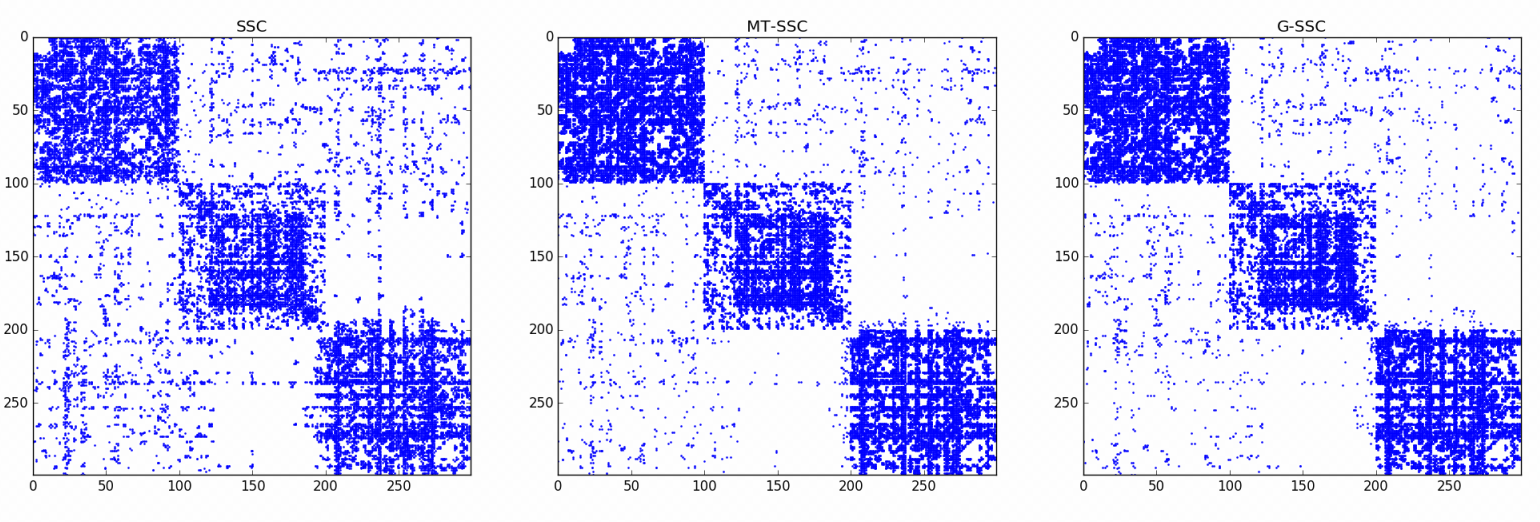
\includegraphics[width=0.8\textwidth]{nus_W}
  \caption{SSC, MT-SSC, G-SSC 在一组测试集上生成的邻接图}
  \label{fig:nus_W}
\end{figure}
\begin{figure}[t!]
  \centering
  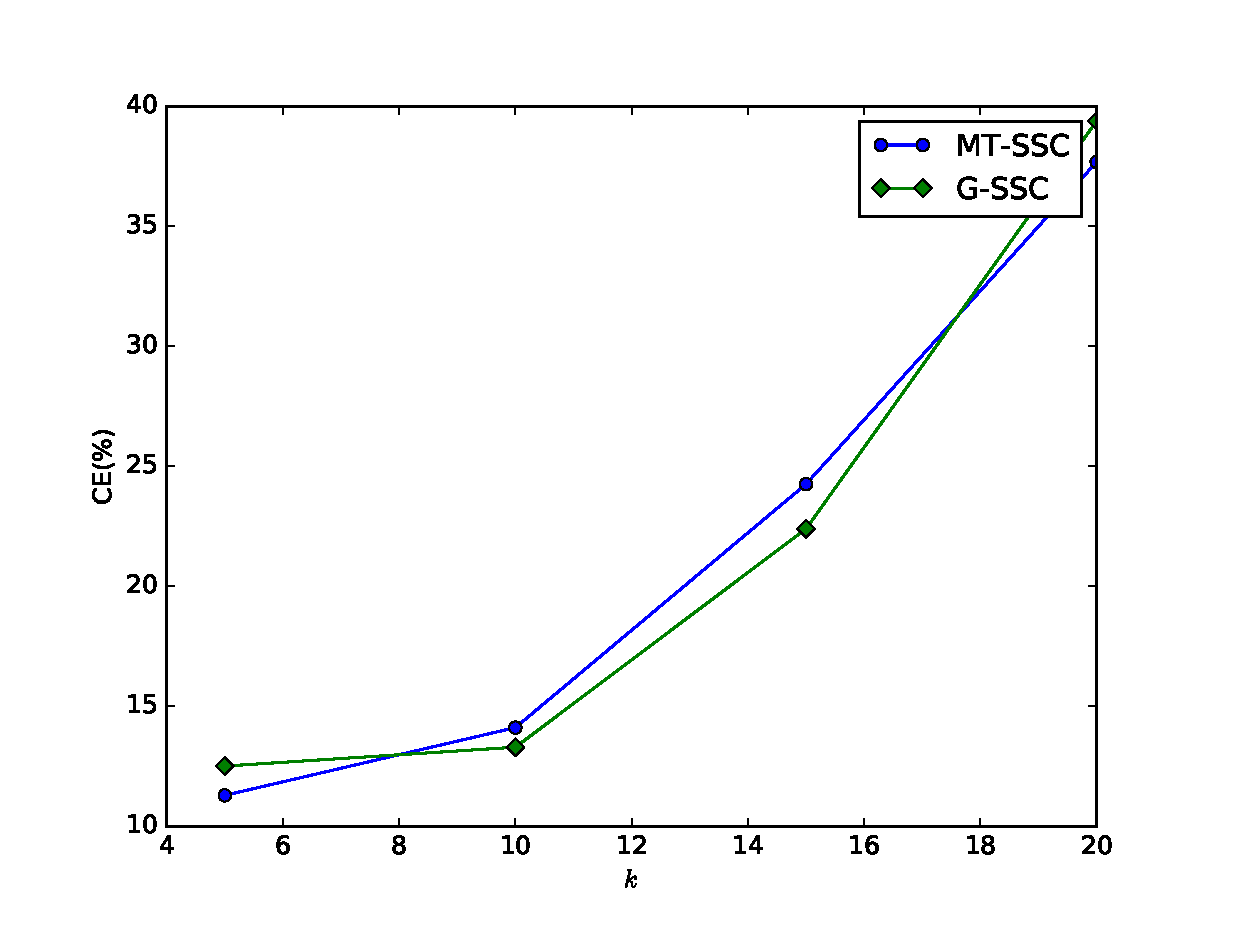
\includegraphics[width=0.6\textwidth]{nus_k}
  \caption{最近邻参数\(k\)对聚类平均错误率的影响}
  \label{fig:nus_k}
\end{figure}
对于分组算法, 同样用PCA将数据降到20维, 并且白化.
取拓展最近邻的参数\(k=5, \theta=0.05, \kappa=0.1\),
得到的分组结果错误率为\(0.0082\), 平均每组包含\(6.42\)个点.
进而对原始数据用MT-SSC和G-SSC算法,
并与SSC比较得到结果如\autoref{tab:nus}.
可以看出MT-SSC、G-SSC 较SSC 聚类正确率更高.
\autoref{fig:nus_W} 是三种算法在某组数据上的邻接图比较,
可以看出MT-SSC和G-SSC比SSC的邻接图错误连接更少,
且同类之间连接更紧密. 我们取了不同的邻居增长参数\(k\)
观察其对聚类结果的影响. 从\autoref{fig:nus_k} 可以看出
最近邻居参数不宜选取的过大, 虽然理论上\autoref{alg:nsn} 
有一定的鲁棒性, 但过大的\(k\)可能会混入很多错误点, 从而
影响阈值\(\theta\)的筛选能力, 并导致自表示发生很大偏差,
降低聚类准确率.

\chapter{总结与展望}
本文介绍了子空间聚类问题, 以及目前公认最有效的方法:
稀疏子空间聚类(SSC)和低秩表示(LRR). 并且列举了基于SSC稀疏自表示思想
的一系列算法. 本文针对SSC的两点不足, 提出了新的多任务和组稀疏子空间聚类方法,
其基本思路是利用数据的局部信息, 将数据点分组. 我们借鉴了~\cite{heckel2013noisy}
中夹角最近邻的想法, 将其推广到投影最近邻, 提出了拓展最近邻算法,
从而将每个点与它在同一局部子空间的点分为一组, 得到指标集族\(\Omega\).
有了分组结果后, 我们提出多任务方法MT-SSC和组稀疏方法G-SSC.
MT-SSC寻求对每个分组内点的同时表示, 而G-SSC将\(\ell_1\)正则化项替换成
\(\ell_{\Omega, 1}\), 以便表示系数相对比较稠密, 从而提升谱聚类的稳定性.

我们对拓展最近邻算法, MT-SSC和G-SSC做了理论分析. 得到在半随机模型下,
如果子空间之间的相关度满足一定条件, 那么拓展最近邻算法第一次循环
加入的点有较大概率和自身在同一子空间. 同时我们还给出了确定性模型下
MT-SSC和G-SSC的表示系数的非零项对应同一子空间中点的条件.
最后我们将新算法在Hopkins155和NUS-WIDE数据集上进行数值实验,
并与SSC、LRR比较. 验证了MT-SSC和G-SSC能在一定的程度上提升聚类结果.

多任务和组稀疏子空间聚类也存在一些问题, 首先分组结果的正确性没有保证,
而如果分组错误, 很可能会对聚类结果带来很大的影响.
其次所需参数过多, 需要给出一些自动选取参数的方法.
最后MT-SSC, G-SSC要求分组互不相交, 然而最近邻集合是有重叠的,
下一步可以考虑利用重叠组稀疏(Overlap Group LASSO)~\cite{jacob2009group},
处理分组有重叠的情形.

另外一个长期困扰自表示类型方法的问题是它们都以观测数据本身作为
字典进行表示, 而观测数据中所含的噪声、缺损、奇异值等都会使字典的
效果下降. 本文作者尝试基于分组结果,用每一组的点得到一个局部的子空间
结构,用每个局部子空间的正交基代替数据本身进行回归表示.如果给定指标集族
\(\Omega=\{\cI_1, \cI_2, \ldots, \cI_{|\Omega|}\}\),
对\(\cI_j\)我们用\(X_{\cI_j}\)的前\(r\)个左奇异向量组成矩阵\(U^{(j)}\)代替\(X_{\cI_j}\).
假设\(i \in \cI_1\), 那么将G-SSC的优化问题换成
\begin{equation}
  \min_{c} \, \|\reshape(c)\|_{2, 1}+\frac{\lambda}{2}
  \left\|x_i-\left[ U^{(2)} U^{(3)} \cdots U^{(|\Omega|)}\right]c\right\|_2^2.
  \label{eq:ussc}
\end{equation}
其中\(\reshape(c)\)是将向量\(c\)的元素\(r\)个一列排成矩阵.
这样字典不再是原始数据而是每类点张成空间的基,在一定程度上可以
使字典更稳定,减少噪音干扰. 不过在Hopkins155 数据集上, \eqref{eq:ussc} 表现不佳,
这可能来由于噪音干扰使得\(U^{(j)}\)中包含了不在自身子空间中方向,
具体原因和改进方法值得进一步探索.

%自行添加
%\input{chapter/...}

%%%%%%%%%%%%%%%%%%%%%%%%%%%%%%
%% 附件部分
%%%%%%%%%%%%%%%%%%%%%%%%%%%%%%
\backmatter

% 参考文献
\bibliography{bib/ref}
%\nocite{*} % for every item

\begin{thanks}
  首先感谢张淑芹导师,没有她的指导和鼓励, 我不可能完成这篇论文. 
  张老师应用驱动的研究思路和对待学术的热忱也将使我受益终身.

  感谢高卫国老师, 在高老师DS \& HPC 讨论班里, 我既能学习经典文献, 
  又有机会接触前沿学术讨论, 极大地提升了自己的专业技能.

  感谢复旦,感谢一路走过来的兄弟姐妹们,在最宝贵年华里,是你们伴随着我的成长.

  最后,感谢我家人一贯的鼓励和支持,你们是我追求学业的坚强后盾.

\end{thanks}
%致谢部分
\makebackcover

\end{document}
